\chapter{Probability}

Luck. Coincidence. Randomness. Uncertainty. Risk. Doubt. Fortune. Chance. You’ve probably heard these words countless times, but chances are that they were
used in a vague, casual way. Unfortunately, despite its ubiquity in science and everyday life, probability can be deeply counterintuitive.

\section{Inspiration and Overview}
\begin{exampleboxbreak}{Probability in Healthcare}
\begin{dialogue}
\speak{RELATIVE} Nurse, what is the probability that the drug will work? \\
\speak{NURSE} I hope it works, we'll know tomorrow. \\
\speak{RELATIVE} Yes, but what is the probability that it will? \\ 
\speak{NURSE} Each case is different, we have to wait. \\
\speak{RELATIVE} But let's see, out of a hundred patients that are treated under similar conditions, how many times would you expect it to work? \\
\speak{NURSE} \emph{(somewhat annoyed)} I told you, every person is different, for some it works, for some it doesn't. \\
\speak{RELATIVE} \emph{(insisting)} Then tell me, if you had to bet whether it will work or not, which side of the bet would you take? \\
\speak{NURSE} \emph{(cheering up for a moment)} I'd bet it will work. \\
\speak{RELATIVE} \emph{(somewhat relieved)} OK, now, would you be willing to lose two dollars if it doesn't work, and gain one dollar if it does? \\
\speak{NURSE} \emph{(exasperated)} What a sick thought! You are wasting my time!
\end{dialogue}
\end{exampleboxbreak}

In this conversation, the relative attempts to use the concept of probability to discuss an uncertain situation—whether the drug will work for their loved one. The nurse's initial responses suggest that the meaning of ``probability'' is not uniformly understood, as they focus on individual differences rather than likelihood. 

The relative tries multiple approaches to make the concept more concrete:
\begin{itemize}
    \item First, requesting a frequency interpretation (``out of a hundred patients\ldots'')
    \item Then, asking for a binary prediction (which side of a bet would the nurse take?)
    \item Finally, attempting to establish specific odds (the two-to-one bet)
\end{itemize}

The nurse may not be entirely wrong in refusing to discuss in such terms—what if this were an experimental drug administered for the very first time in this hospital or in the nurse's experience? 

This dialogue exemplifies how probability can be viewed through different lenses: as statistical frequencies based on past events, or as subjective beliefs about unique circumstances. The relative's final attempt to establish a bet based on these probabilities reveals an important application of probability theory—decision-making under uncertainty and risk assessment. The nurse's discomfort with this proposition highlights how probability concepts, while mathematically sound, can create social friction when applied to medical contexts where uncertainty is typically managed through standardized protocols rather than explicit probability assessments.

\headingA{Frequency vs. Subjective Interpretations}

While there are many situations involving uncertainty in which the frequency interpretation is appropriate, there are other situations where it is not applicable. Consider, for example, a scholar who asserts that the Iliad and the Odyssey were composed by the same person, with probability 90\%. Such an assertion conveys meaningful information, but not in terms of frequencies, since the subject is a one-time historical event. Rather, it is an expression of the scholar's subjective belief based on evidence and expertise.

\headingA{The Importance of Subjective Probability}

One might initially dismiss subjective beliefs as uninteresting from a mathematical or scientific perspective. However, people frequently make choices in the presence of uncertainty, and a systematic framework for utilizing these beliefs is essential for successful—or at least consistent—decision making.

\headingA{Probability in Action}

This distinction between frequency-based and subjective interpretations highlights the versatility of probability theory. In the opening dialogue, we see both interpretations at work:
\begin{itemize}
    \item The relative first seeks a frequency-based answer (``out of a hundred patients'')
    \item Then pivots to eliciting the nurse's subjective belief about this particular treatment's effectiveness
\end{itemize}

Had the nurse been willing to accept a one-for-one bet that the drug would work, we could infer that the nurse judged the probability of success to be at least \(50\%\). Had the nurse accepted the final proposed bet (two-for-one), this would have indicated a success probability of at least \(2/3\).

\section{Set Theory Review}

\begin{definitionboxbreak}{Set}
A set is a collection of distinct objects, considered as an object in its own right.
\begin{itemize}
    \item Sets are typically denoted by curly braces, e.g., \( S = \{1, 2, 3\} \).
    \item The objects within a set are called elements or members. For example, in the set \( S \), the number \( 1 \) is an element of \( S \), denoted as \( 1 \in S \) and if \( 4 \) is not in \( S \), we write \( 4 \notin S \).
    \item A set can have any number of elements, including none (the empty set, denoted \( \emptyset \)).
    \item If \(S\) contains a finite number of elements, we say \(S = \{1,2,3\}\) is a finite set.
    \item If \(S\) contains infinite elements, such as the set of all natural numbers \( \mathbb{N} = \{1, 2, 3, \ldots\} \), we say \(S\) is countably infinite.
\end{itemize}

\end{definitionboxbreak}

\newcommand{\circled}[1]{\tikz[baseline=(char.base)]{
            \node[shape=circle,draw,inner sep=1pt] (char) {#1};}}
            
\begin{keyconceptboxbreak}{Countable Infinity vs. Uncountably Infinite Sets}

    \headingB{Countably Infinite Sets:}
    \begin{definitionboxbreak}{Countably Infinite}
    A set $S$ is \textbf{countably infinite} if its elements can be put into a one-to-one correspondence (bijection) with the natural numbers $\mathbb{N} = \{1, 2, 3, \ldots\}$. In other words, the elements of $S$ can be arranged in a sequence: $s_1, s_2, s_3, \ldots$ where every element of $S$ appears exactly once in the sequence.
    \end{definitionboxbreak}
    
    The term ``countable'' refers to both finite sets and countably infinite sets, meaning we can count their elements one by one (even if the counting process never ends).

    \headingB{Examples of Countably Infinite Sets:}
    \begin{itemize}
        \item The set of integers $\mathbb{Z} = \{\ldots, -2, -1, 0, 1, 2, \ldots\}$ is countably infinite.
        \item The set of rational numbers $\mathbb{Q} = \{\frac{p}{q} : p, q \in \mathbb{Z}, q \neq 0\}$ is countably infinite.
    \end{itemize}

    \headingB{Uncountably Infinite Sets:}
    \begin{definitionboxbreak}{Uncountably Infinite}
    A set $S$ is \textbf{uncountably infinite} if it is infinite but cannot be put into a one-to-one correspondence with the natural numbers $\mathbb{N}$. In other words, the elements of $S$ cannot be arranged in a sequence where each element appears exactly once.
    \end{definitionboxbreak}
    
    Uncountable sets represent a ``larger'' kind of infinity than countable sets. The existence of different sizes of infinity was one of Cantor's most revolutionary discoveries.

    \headingB{Examples of Uncountable Sets:}
    \begin{itemize}
        \item The set of real numbers $\mathbb{R}$ is uncountably infinite.
        \item The set of all functions $f: \mathbb{N} \rightarrow \{0,1\}$ is uncountably infinite.
        \item The set of irrational numbers is uncountably infinite.
    \end{itemize}
\end{keyconceptboxbreak}

\begin{funfactsbreak}{Cantor's Infinite Hotel}

\headingB{Did you know?} There are different sizes of infinity! Georg Cantor proved this mind-bending fact in the 1870s, shocking the mathematical world.

\headingB{Imagine a Hotel with Infinite Rooms:}

\infoheading{Scenario 1:} The infinite hotel is full, but one new guest arrives. Can you accommodate them?

\infoheading{Solution:} Yes! Ask each guest to move from room $n$ to room $n+1$. This frees up room 1 for the new guest!

\infoheading{Scenario 2:} The infinite hotel is full, and a bus with infinite new guests arrives. Can you fit them all?

\infoheading{Solution:} Yes! Ask each current guest to move from room $n$ to room $2n$. This puts all current guests in even-numbered rooms, leaving all odd-numbered rooms free for the infinitely many new guests!

\headingB{Counting Rational Numbers}

Surprisingly, all rational numbers can be accommodated in our Infinite Hotel! They are what mathematicians call ``countably infinite''.

\begin{figure}[H]
    \centering
    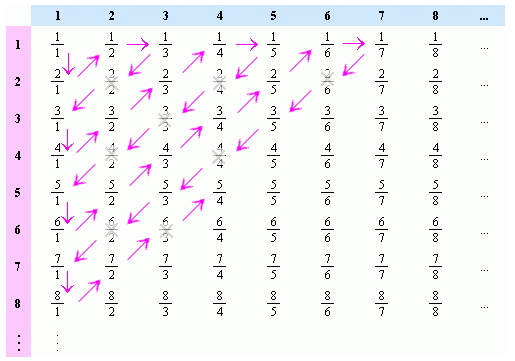
\includegraphics[width=0.6\textwidth]{cantor_diag.png}
    \caption{Cantor's diagonal zigzag method for counting rational numbers}
    \label{fig:cantor_diag}
\end{figure}

\infoheading{Key Insight:} Cantor's diagonal zigzag pattern (shown in Figure~\ref{fig:cantor_diag}) creates a one-to-one correspondence between natural numbers and rational numbers. This clever counting method ensures we'll eventually reach any specific fraction after a finite number of steps, proving that rational numbers are countable—they can all fit in our Infinite Hotel!

\headingB{But Irrational Numbers Won't Fit!}

Cantor discovered that the real numbers (which include both rational and irrational numbers) form an \textit{uncountable} infinity. Here's why:


\headingB{The Diagonal Argument: Why Real Numbers Won't Fit}
To fully appreciate what ``countable'' means, it's crucial to see Cantor's proof that some infinite sets are uncountable. The most famous example is the set of real numbers ($\mathbb{R}$) between 0 and 1. An uncountable set is an infinite set for which no one-to-one correspondence with the natural numbers can ever be made.

\headingB{The Proof by Contradiction}

\headingB{Assume the Opposite}
Let's assume the set of real numbers between 0 and 1 is countable. If it's countable, we can write them all down in an infinite list, just like we did for the rationals. Let this hypothetical list be:
\begin{align*}
r_1 &= 0.\mathbf{d_{11}}d_{12}d_{13}d_{14}\dots \\
r_2 &= 0.d_{21}\mathbf{d_{22}}d_{23}d_{24}\dots \\
r_3 &= 0.d_{31}d_{32}\mathbf{d_{33}}d_{34}\dots \\
r_4 &= 0.d_{41}d_{42}d_{43}\mathbf{d_{44}}\dots \\
&\vdots
\end{align*}
..and so on, where $d_{ij}$ is the $j$-th decimal digit of the $i$-th number.

\headingB{Construct a New Number}
Now, we'll construct a new real number, let's call it $X$, which is \emph{not} on this list. We do this by going down the diagonal of our list (the bold digits) and changing each digit.
\begin{itemize}
\item The first decimal digit of $X$ will be different from the first digit of $r_1$ ($d_{11}$).
\item The second decimal digit of $X$ will be different from the second digit of $r_2$ ($d_{22}$).
\item The third decimal digit of $X$ will be different from the third digit of $r_3$ ($d_{33}$).
\item In general, the $n$-th digit of $X$ is different from the $n$-th digit of $r_n$.
\end{itemize}
Let's define a rule: If the diagonal digit $d_{nn}$ is 1, we make our new digit 2. If $d_{nn}$ is anything else, we make our new digit 1.

\paragraph{Example:}
Suppose our list starts like this:
\begin{align*}
r_1 &= 0.\mathbf{7}182\dots \\
r_2 &= 0.3\mathbf{1}41\dots \\
r_3 &= 0.88\mathbf{2}3\dots \\
r_4 &= 0.413\mathbf{5}\dots
\end{align*}
Our new number $X$ is constructed as follows:
\begin{itemize}
\item 1st digit of $X$ is not 7 (let's make it 1).
\item 2nd digit of $X$ is not 1 (let's make it 2).
\item 3rd digit of $X$ is not 2 (let's make it 1).
\item 4th digit of $X$ is not 5 (let's make it 1).
\end{itemize}
So, $X = 0.1211\dots$

\headingB{The Contradiction}
This new number $X$ is a real number between 0 and 1. But where is it on our list?
\begin{itemize}
\item It can't be $r_1$ because its first digit is different.
\item It can't be $r_2$ because its second digit is different.
\item It can't be $r_n$ for any $n$, because its $n$-th digit is different from $r_n$'s $n$-th digit.
\end{itemize}
So, $X$ is \textbf{not on the list}. But we started by assuming our list contained \emph{all} real numbers between 0 and 1. This is a contradiction.

\headingB{Conclusion}
Our initial assumption must be false. It is impossible to list all the real numbers between 0 and 1. Therefore, the set of real numbers is \textbf{uncountably infinite}. It represents a ``larger'' infinity than the infinity of integers or rational numbers.

\end{funfactsbreak}

\subsection{Set Operations}
We will denote the \textbf{universal set} by \( \Omega \), which contains all possible outcomes or elements under consideration. Subsets of \( \Omega \) are denoted by capital letters such as \( A \), \( B \), and \( C \).
The \textbf{complement} of a set \( S \), denoted \( S^c \) or \( \overline{S} \), is the set of all elements in the universal set \( \Omega \) that are not in \( S \):

\[
S^c = \{ x \in \Omega \mid x \notin S \}
\]
\[ \Omega^c = \emptyset   \]

The \textbf{union} of two sets \( A \) and \( B \), denoted \( A \cup B \), is the set of elements that are in \( A \), in \( B \), or in both:

\[
A \cup B = \{ x \mid x \in A \text{ or } x \in B \}
\]

The \textbf{intersection} of two sets \( A \) and \( B \), denoted \( A \cap B \), is the set of elements that are in both \( A \) and \( B \):

\[
A \cap B = \{ x \mid x \in A \text{ and } x \in B \}
\]

The \textbf{set difference} of \( A \) and \( B \), denoted \( A \setminus B \), is the set of elements that are in \( A \) but not in \( B \):

\[
A \setminus B = \{ x \mid x \in A \text{ and } x \notin B \} = A \cap B^c
\]

The \textbf{symmetric difference} of \( A \) and \( B \), denoted \( A \triangle B \), is the set of elements that are in exactly one of the sets \( A \) or \( B \):

\[
A \triangle B = (A \setminus B) \cup (B \setminus A) = (A \cup B) \setminus (A \cap B)
\]


% Include the combined set operations diagram generated with matplotlib
\begin{figure}[h]
    \centering
    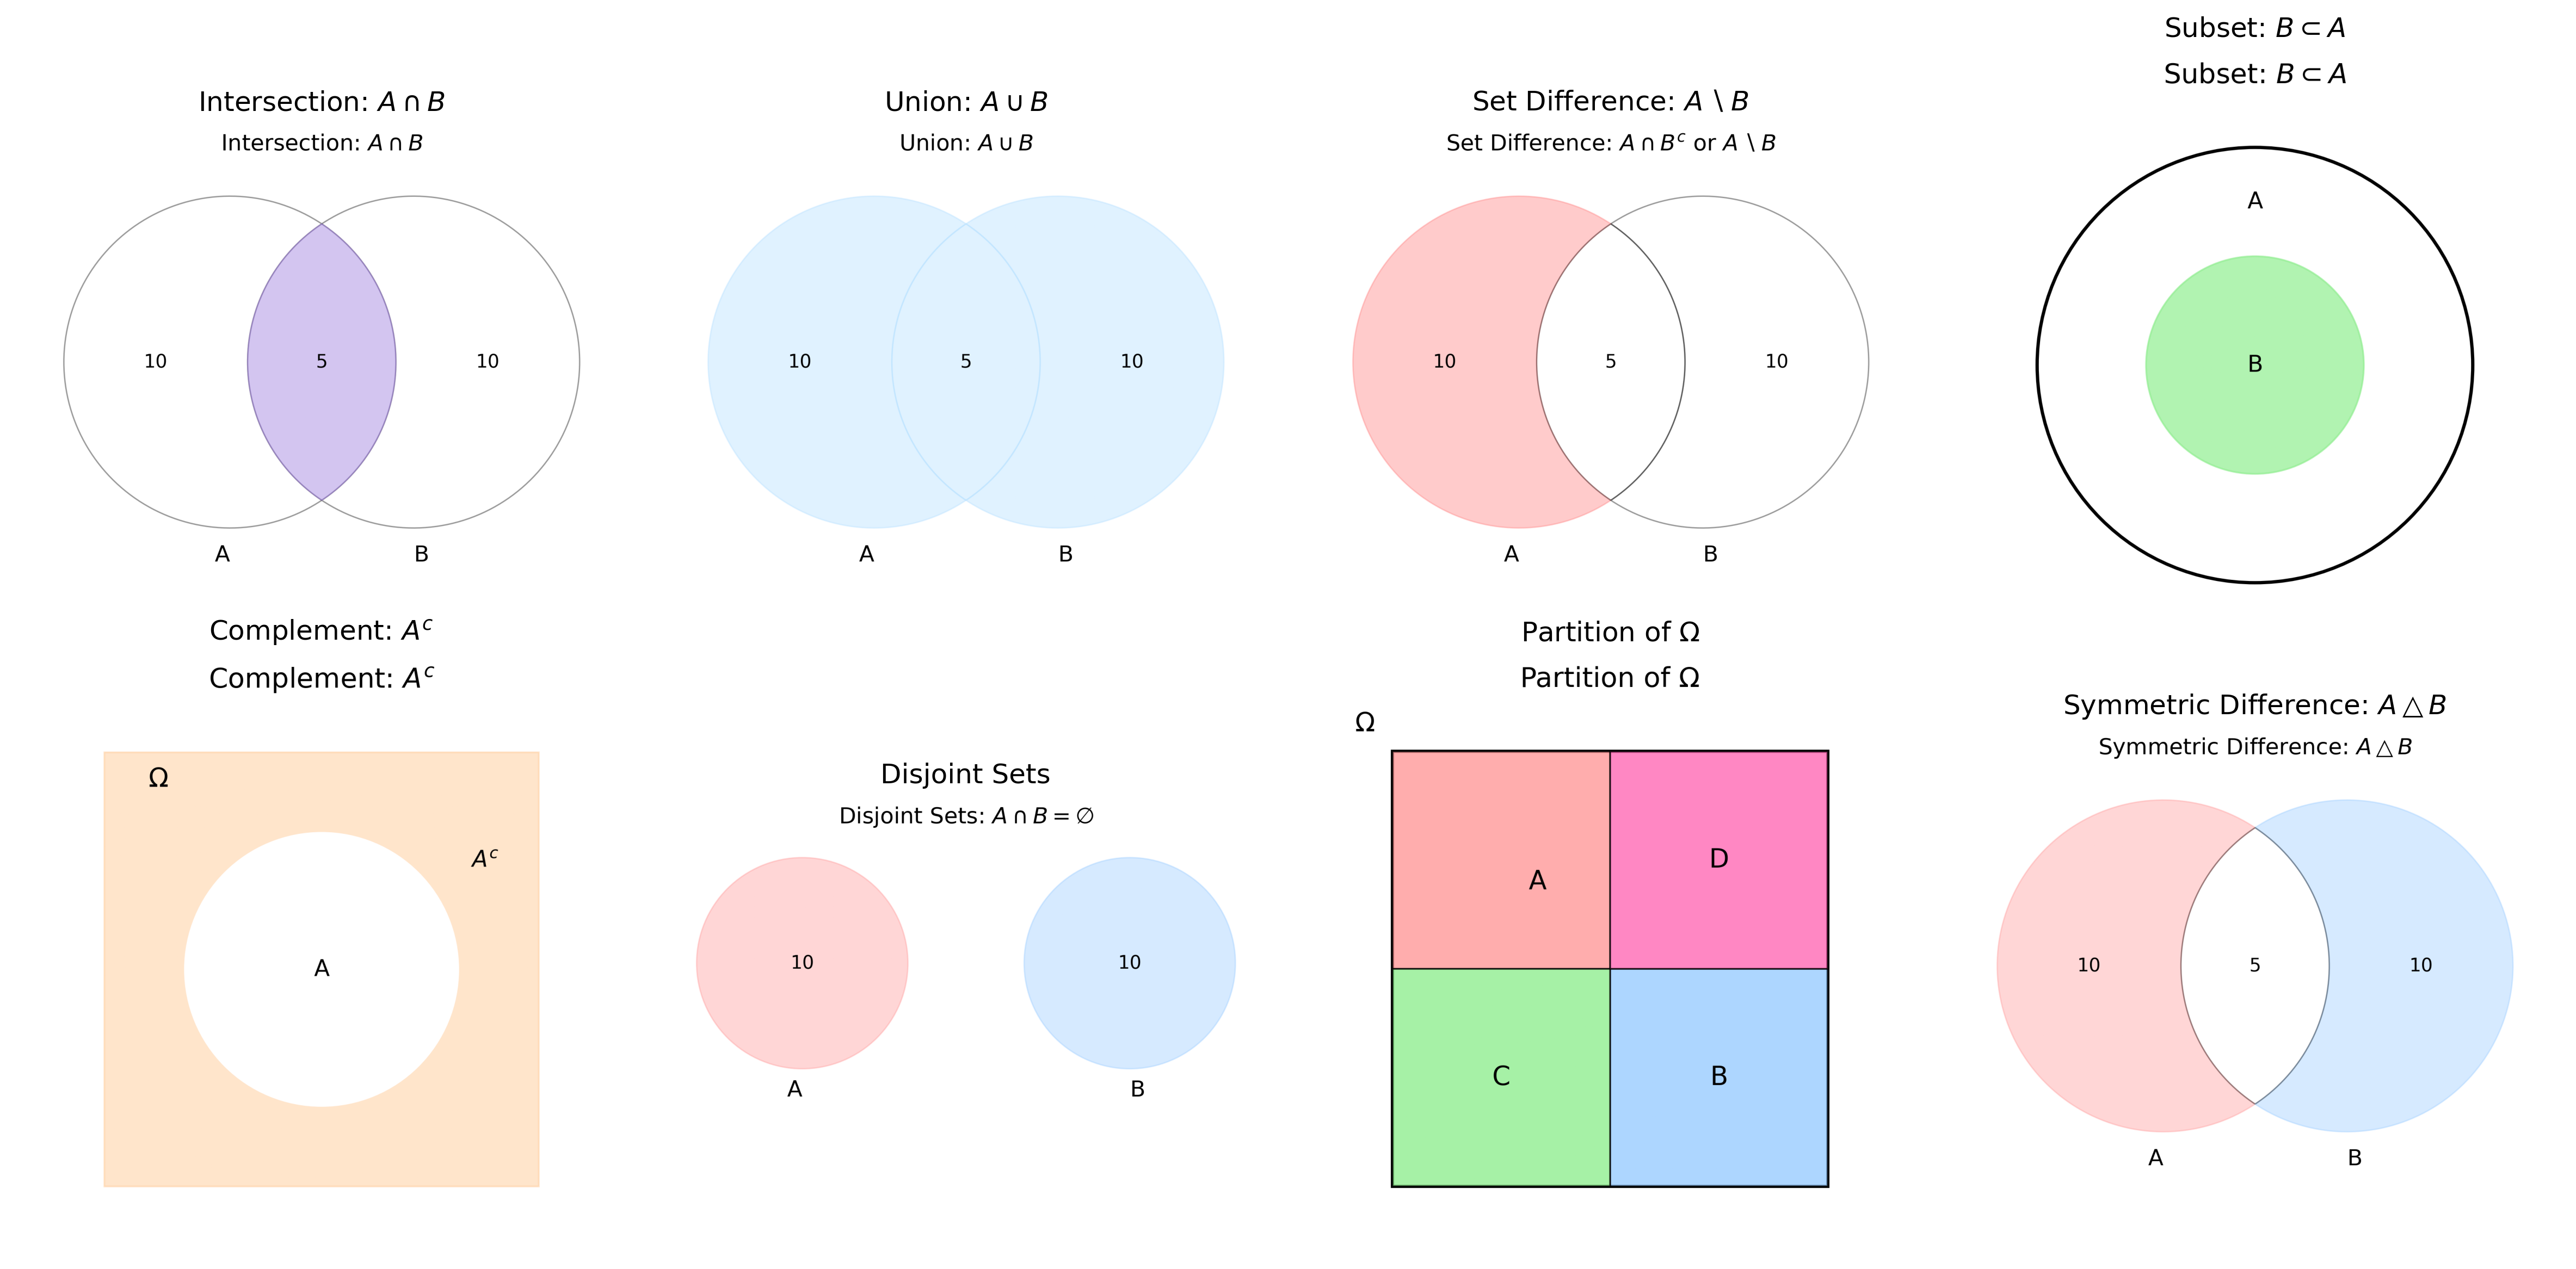
\includegraphics[width=\textwidth]{figures/set_operations/all_operations.png}
    \caption{Visualizations of fundamental set operations}\label{fig:set_operations}
\end{figure}

The union or intersection of more or infinitely many sets is defined similarly. For example, the union of a collection of sets \( \{A_i\}_{i \in I} \) is:

\[
\bigcup_{i \in I} A_i = \{ x \mid x \in A_i \text{ for some } i \in I \}
\]

And the intersection is:

\[
\bigcap_{i \in I} A_i = \{ x \mid x \in A_i \text{ for all } i \in I \}
\]

If two sets \( A \) and \( B \) have no elements in common, they are called \textbf{disjoint}, and their intersection is the empty set:
\[ A \cap B = \emptyset \]  

A collection of sets \( \{A_i\}_{i \in I} \) is called a \textbf{partition} of a set \( S \) if:
\begin{itemize}
    \item The sets \( A_i \) are pairwise disjoint: \( A_i \cap A_j = \emptyset \) for all \( i \neq j \)
    \item The union of all sets in the collection equals \( S \): \( \bigcup_{i \in I} A_i = S \)
\end{itemize}   

% \begin{figure}[h]
%     \centering
%     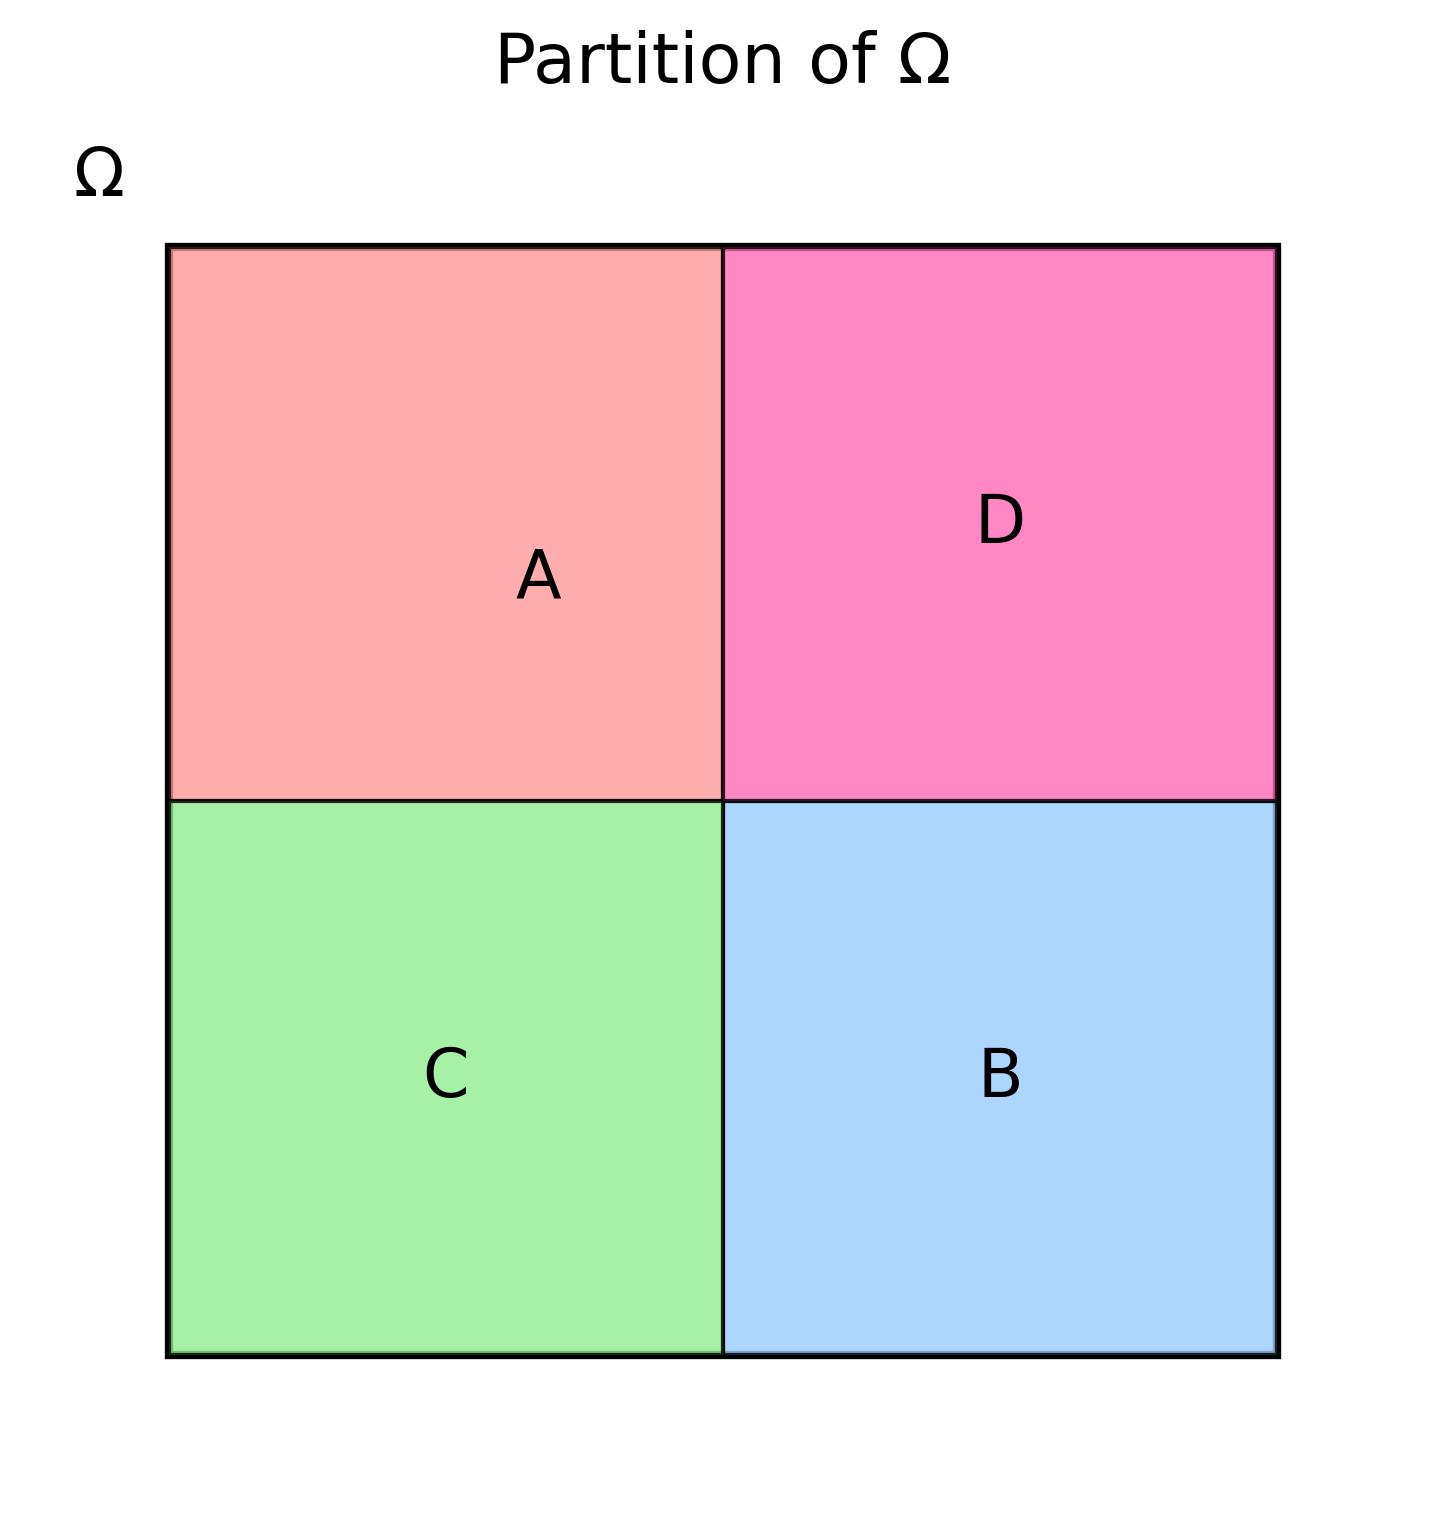
\includegraphics[width=0.6\textwidth]{figures/set_operations/partition.png}
%     \caption{A partition of a set: disjoint subsets whose union equals the whole set}\label{fig:set-partition}
% \end{figure}

\subsubsection{Set Algebra}

\begin{identitiesboxbreak}{Set Theory}
For any sets \( A \), \( B \), and \( C \) within a universal set \( \Omega \), the following identities hold:
\begin{itemize}
    \item \textbf{Commutative Laws:}
    \[ A \cup B = B \cup A \]
    \[ A \cap B = B \cap A \]
    \item \textbf{Associative Laws:}
    \[ (A \cup B) \cup C = A \cup (B \cup C) \]
    \[ (A \cap B) \cap C = A \cap (B \cap C) \]
    \item \textbf{Distributive Laws:}
    \[ A \cup (B \cap C) = (A \cup B        ) \cap (A \cup C) \]
    \[ A \cap (B \cup C) = (A \cap B) \cup (A \cap C) \]
    \item \textbf{Identity Laws:}
    \[ A \cup \emptyset = A \]
    \[ A \cap \Omega = A \]
    \item \textbf{Domination Laws:}
    \[ A \cup \Omega = \Omega \]        
    \[ A \cap \emptyset = \emptyset \]      
    \item \textbf{Idempotent Laws:}
    \[ A \cup A = A \]
    \[ A \cap A = A \]
    \item \textbf{Complement Laws:}
    \[ A \cup A^c = \Omega \]
    \[ A \cap A^c = \emptyset \]
    \item \textbf{Double Complement Law:}
    \[ (A^c)^c = A \]
    \item \textbf{De Morgan's Laws:}
    \[ (A \cup B)^c = A^c \cap B^c \]
    \[ (A \cap B)^c = A^c \cup B^c \]
\end{itemize}
\end{identitiesboxbreak}

\section{Probablistic Models}

Probability is a mathematical descrption of an unknown phenomenon. It is used to predict the likelihood of various outcomes. A probablistic model consists of three main components:
\begin{itemize}
    \item A \textbf{sample space} \( \Omega \), which is the set of all possible outcomes.
    \item A set of \textbf{events}, which are subsets of the sample space.
    \item A \textbf{probability measure/probability law} \( P \), which assigns to a set \(A\) of possible outcomes called an event , a non negative number \( P(A) \) called the probability of \(A\) that encodes our knowledge or belief about the collective likelihood of the elements of \(A\). 

\subsection{Sample Space and Events}
\begin{itemize}
    \item Every probabilistic model involves an underlying process, called the \textbf{experiment}, that will produce exactly one out of several possible \textbf{outcomes}.
    \item The set of all possible outcomes is called the \textbf{sample space}, denoted by \( \Omega \).
    \item An \textbf{event} is any subset of the sample space, including the empty set and the sample space itself.
    \item Events can be combined using set operations such as union, intersection, and complement.
\end{itemize}

\subsubsection{Choosing a Sample Space}
When defining a probabilistic model, the choice of sample space is crucial. The sample space should:
\begin{itemize}
    \item Include all possible outcomes of the experiment.
    \item Be as specific as necessary for the problem at hand.
    \item Allow for the definition of all relevant events.
\end{itemize}

\begin{exampleboxbreak}{Choosing a Sample Space}
\headingB{Example 1: Rolling a Die}
\begin{itemize}
    \item Experiment: Rolling a fair six-sided die.
    \item Sample Space: \( \Omega = \{1, 2, 3, 4, 5, 6\} \).
    \item Events:
    \begin{itemize}
        \item \( A = \{2, 4, 6\} \) (rolling an even number)
        \item \( B = \{1, 3, 5\} \) (rolling an odd number)
        \item \( C = \{1, 2\} \) (rolling a number less than 3)
    \end{itemize}
\end{itemize}   
\headingB{Example 2: Flipping a Coin}
\begin{itemize}
    \item Experiment: Flipping a fair coin.
    \item Sample Space: \( \Omega = \{\text{Heads}, \text{Tails}\} \).
    \item Events:
    \begin{itemize}
        \item \( A = \{\text{Heads}\} \) (getting heads)
        \item \( B = \{\text{Tails}\} \) (getting tails)
    \end{itemize}
\end{itemize}
\headingB{Example 3: Drawing a Card from a Deck}
\begin{itemize} 
    \item Experiment: Drawing a card from a standard deck of 52 playing cards.
    \item Sample Space: \( \Omega = \{\text{2H}, \text{3H}, \ldots, \text{AH}, \text{2D}, \ldots, \text{AD}, \text{2C}, \ldots, \text{AC}, \text{2S}, \ldots, \text{AS}\} \) (where H, D, C, S represent hearts, diamonds, clubs, and spades respectively).
    \item Events:
    \begin{itemize}
        \item \( A = \{\text{All Hearts}\} = \{\text{2H}, \text{3H}, \ldots, \text{AH}\} \)
        \item \( B = \{\text{All Face Cards}\} = \{\text{JH}, \text{QH}, \text{KH}, \text{JD}, \text{QD}, \text{KD}, \text{JC}, \text{QC}, \text{KC}, \text{JS}, \text{QS}, \text{KS}\} \)
        \item \( C = \{\text{All Aces}\} = \{\text{AH}, \text{AD}, \text{AC}, \text{AS}\} \)
    \end{itemize}
\end{itemize}
\end{exampleboxbreak}

\subsubsection{Properties of a Well-Defined Sample Space}

A properly defined sample space must satisfy certain requirements to be useful in probabilistic modeling:

\begin{itemize}
    \item \textbf{Mutually Exclusive Outcomes}: Each outcome in the sample space must be distinct and non-overlapping. The outcomes must be defined so that when the experiment is conducted, exactly one outcome occurs.
    
    \item \textbf{Collectively Exhaustive Outcomes}: The sample space must include all possible outcomes of the experiment.
    
    \item \textbf{Appropriate Level of Detail}: The sample space should be defined with enough detail to answer the questions of interest, but not so detailed as to make the analysis unnecessarily complex.
\end{itemize}

\begin{exampleboxbreak}{Finding the Right Level of Detail in a Sample Space}
Consider a clinical trial testing the effectiveness of a new drug. Three possible approaches to defining the sample space illustrate the importance of choosing an appropriate level of detail:

\headingB{Approach 1: Too Little Detail}
\[ \Omega_1 = \{\text{``Drug works''}, \text{``Drug doesn't work''}\} \]

This sample space lacks sufficient detail because:
\begin{itemize}
    \item It doesn't capture varying degrees of effectiveness
    \item It ignores potential side effects
    \item It doesn't account for different patient responses
    \item It can't answer questions about the magnitude of improvement
\end{itemize}

\headingB{Approach 2: Too Much Detail}
\begin{align*}
\Omega_2 = \{\text{``Every possible molecular interaction in each patient''}\}
\end{align*}

This sample space has excessive detail because:
\begin{itemize}
    \item It includes information irrelevant to the drug's effectiveness
    \item It makes probability calculations practically impossible
    \item It obscures the clinically relevant outcomes
    \item It introduces unnecessary complexity that doesn't help answer the core question
\end{itemize}

\headingB{Approach 3: Appropriate Level of Detail}
\begin{align*}
\Omega_3 = \{\text{``No effect''}, \text{``Mild improvement''}, \text{``Moderate improvement''}, \\ 
\text{``Major improvement''}, \text{``Adverse reaction''}\}
\end{align*}

This sample space balances detail with practicality:
\begin{itemize}
    \item It captures clinically meaningful outcome categories
    \item It includes sufficient detail to evaluate effectiveness
    \item It allows for statistical analysis of results
    \item It directly addresses the question of interest without unnecessary complexity
\end{itemize}
\end{exampleboxbreak}

\begin{exampleboxbreak}{Improper Sample Space Definition}
Consider the roll of a standard six-sided die. The following would be an improper sample space:
\begin{align*}
\Omega = \{\text{``1 or 3''}, \text{``1 or 4''}, \text{``2''}, \text{``3''}, \text{``5''}, \text{``6''}\}
\end{align*}

This is improper because:
\begin{itemize}
    \item If the roll results in 1, we wouldn't know whether the outcome is ``1 or 3'' or ``1 or 4''
    \item The outcomes are not mutually exclusive (they overlap)
    \item When a specific experimental result occurs (e.g., rolling a 1), the outcome wouldn't be uniquely determined
\end{itemize}

A proper sample space for this experiment would be:
\[ \Omega = \{1, 2, 3, 4, 5, 6\} \]

With this definition, each possible roll corresponds to exactly one outcome in the sample space.
\end{exampleboxbreak}
\begin{exampleboxbreak}{Sample Space Design: Two Coin Flipping Games}
Consider two alternative games, both involving ten successive coin tosses:

\headingB{Game 1:} We receive \$1 each time a head comes up.

\headingB{Game 2:} We receive \$1 for every coin toss, up to and including the first time a head comes up. Then, we receive \$2 for every coin toss, up to the second time a head comes up. More generally, the dollar amount per toss is doubled each time a head comes up.

These games illustrate how the same experiment can be modeled with different levels of detail depending on what information we need:

\headingB{The Underlying Sample Space}
Both games involve the same physical experiment: ten successive coin tosses. The complete sample space for this experiment is:
\[ \Omega = \{\text{all possible sequences of H and T of length 10}\} \]
This sample space has $2^{10} = 1024$ possible outcomes.

\headingB{Sample Space for Game 1}
In Game 1, only the total number of heads matters, not their positions in the sequence. We can use a \textbf{simplified sample space}:
\[ \Omega_1 = \{0, 1, 2, \ldots, 10\} \]
where each outcome represents the number of heads obtained in the ten tosses. This simplified space has only 11 outcomes and is sufficient for calculating payouts in Game 1, since all sequences with the same number of heads yield the same payout.

\headingB{Sample Space for Game 2}
For Game 2, the order of heads and tails is crucial because payouts depend on when heads appear. We must use the complete sample space:
\[ \Omega_2 = \{\text{all possible sequences of H and T of length 10}\} \]

For example, the sequences HHTTTHTHTT and HTHTTTTHTH would yield different payouts in Game 2, even though both contain exactly 4 heads. According to the rules, we receive a payment for every coin toss, and the amount per toss doubles each time a head appears. 

For the sequence HHTTTHTHTT:
\begin{itemize}
    \item Toss 1 (H): \$1 (first head appears, rate becomes \$2 for subsequent tosses)
    \item Toss 2 (H): \$2 (second head appears, rate becomes \$4 for subsequent tosses)
    \item Toss 3 (T): \$4
    \item Toss 4 (T): \$4
    \item Toss 5 (T): \$4
    \item Toss 6 (H): \$4 (third head appears, rate becomes \$8 for subsequent tosses)
    \item Toss 7 (T): \$8
    \item Toss 8 (H): \$8 (fourth head appears, rate becomes \$16 for subsequent tosses)
    \item Toss 9 (T): \$16
    \item Toss 10 (T): \$16
\end{itemize}
Total: \$1 + \$2 + \$4 + \$4 + \$4 + \$4 + \$8 + \$8 + \$16 + \$16 = \$67.

For the sequence HTHTTTTHTH:
\begin{itemize}
    \item Toss 1 (H): \$1
    \item Toss 2 (T): \$2
    \item Toss 3 (H): \$2
    \item Toss 4 (T): \$4
    \item Toss 5 (T): \$4
    \item Toss 6 (T): \$4
    \item Toss 7 (T): \$4
    \item Toss 8 (H): \$4
    \item Toss 9 (T): \$8
    \item Toss 10 (H): \$8
\end{itemize}
Total: \$1 + \$2 + \$2 + \$4 + \$4 + \$4 + \$4 + \$4 + \$8 + \$8 = \$41.

Even though both sequences have the same number of heads, they yield different payouts (\$67 vs \$41) because the positions of the heads differ.

\headingB{Key Insight: Choosing the Right Level of Detail}

Both games share the same underlying sample space (all 1024 possible sequences), but we model them differently:
\begin{itemize}
    \item \textbf{Game 1:} We can use the simplified sample space $\Omega_1$ with only 11 outcomes because multiple sequences (those with the same number of heads) produce identical payouts. This simplification makes calculations much easier.

    \item \textbf{Game 2:} We must use the complete sample space $\Omega_2$ with all 1024 sequences because each distinct sequence may produce a different payout.
\end{itemize}

\headingB{General Principle}

This example demonstrates an important principle in probability modeling: \textbf{The sample space should contain enough detail to distinguish between outcomes that matter for your problem, but no more.}

\begin{itemize}
    \item Too little detail $\rightarrow$ Cannot answer your questions correctly
    \item Too much detail $\rightarrow$ Makes calculations unnecessarily complex
    \item Just right $\rightarrow$ Simplifies work while preserving all relevant information
\end{itemize}

For Game 1, the simplified space $\Omega_1$ is "just right" because all sequences with the same head count are equivalent for our purposes. For Game 2, we need the full detail of $\Omega_2$ to distinguish between different sequences.
\end{exampleboxbreak}


\section{Sequential Models}

Many experiments have an inherently sequential character, such as for example tossing a coin three times, or observing the value of a stock on five successive days, or receiving eight successive digits at a communication receiver. It is then often useful to describe the experiment and the associated sample space by means of a tree-based sequential description.

\subsection{Tree-Based Sequential Description}

A \textbf{tree diagram} provides a visual representation of sequential experiments, where:
\begin{itemize}
    \item Each branch represents a possible outcome at a particular stage
    \item The path from the root to a leaf represents a complete sequence of outcomes
    \item The set of all paths (leaves) forms the sample space
\end{itemize}


Consider the experiment of tossing a fair coin three times. Each toss can result in either Heads (H) or Tails (T). The sample space can be represented as a tree:

\begin{figure}[h]
    \centering
    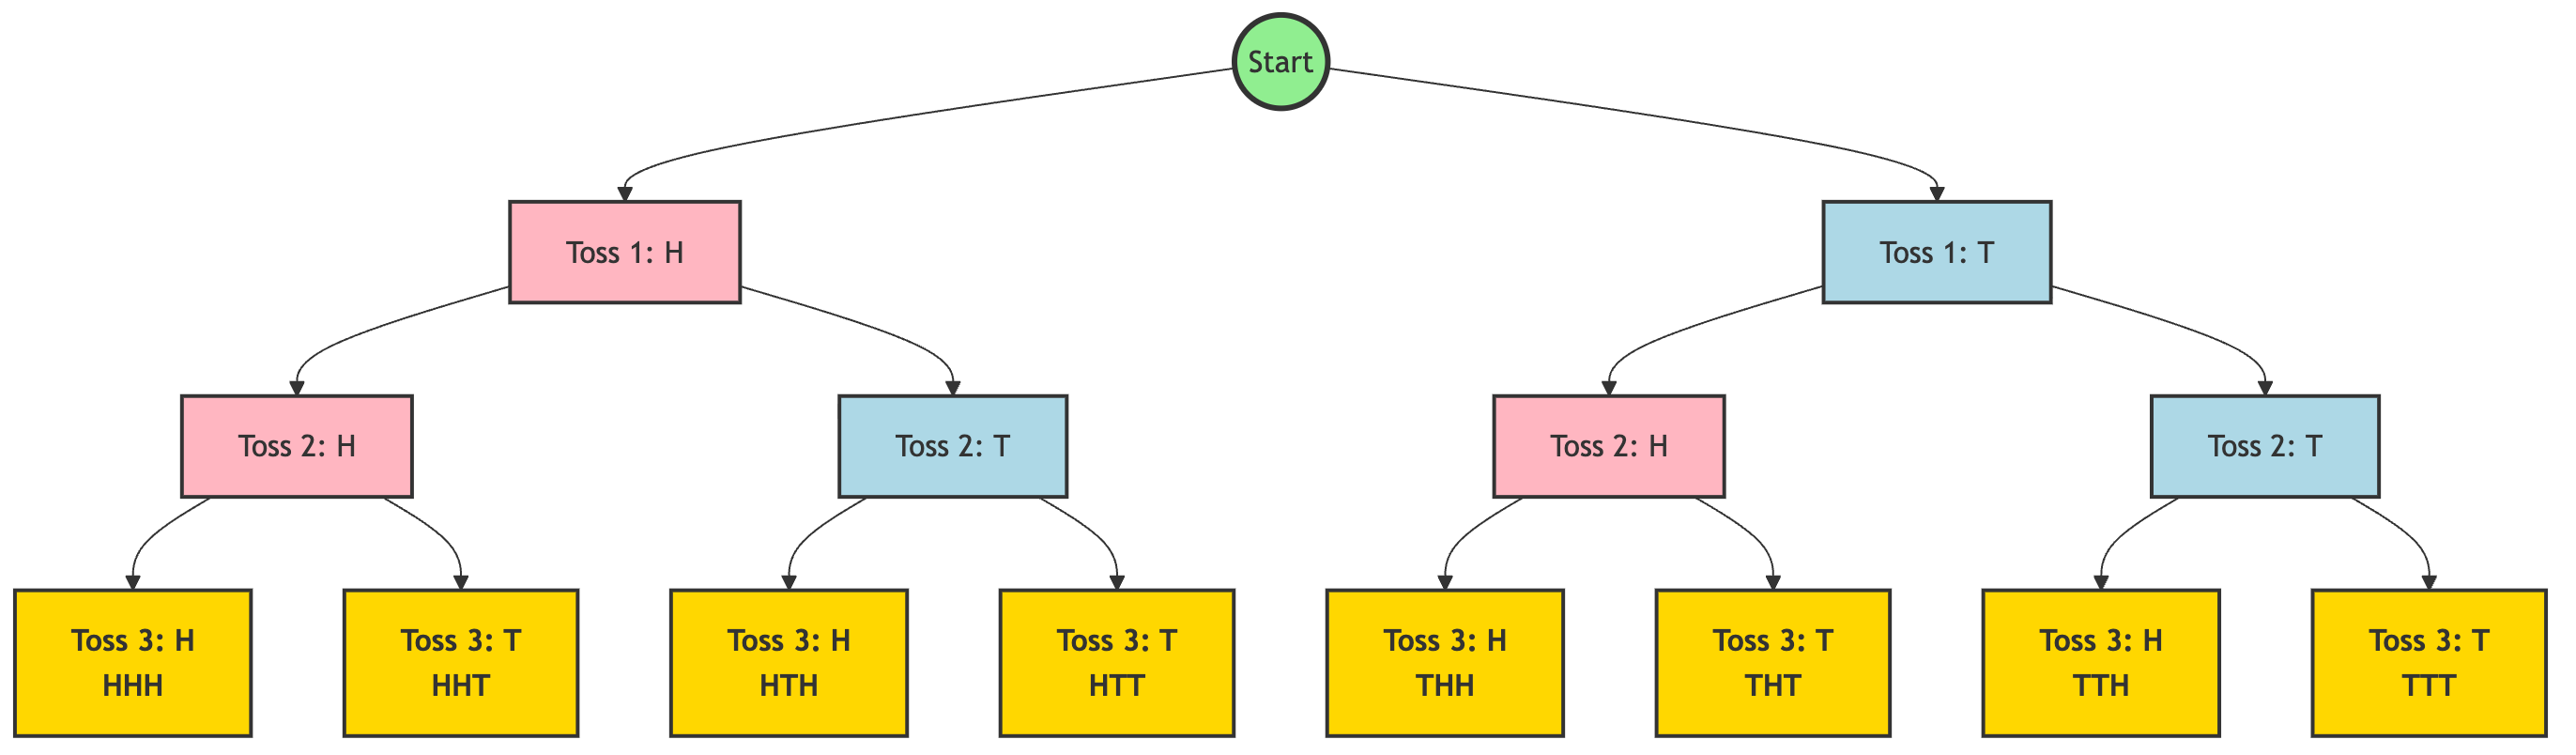
\includegraphics[width=0.9\textwidth]{sequential_tree.png}
    \caption{Tree diagram for three successive coin tosses}
    \label{fig:sequential_tree}
\end{figure}

\headingB{Reading the Tree:}
\begin{itemize}
    \item \textbf{Stage 1 (First Toss):} Two branches from the start—one for H and one for T
    \item \textbf{Stage 2 (Second Toss):} From each outcome of the first toss, two more branches emerge
    \item \textbf{Stage 3 (Third Toss):} From each outcome of the second toss, two final branches complete the sequences
\end{itemize}

\headingB{Sample Space:}
The complete sample space consists of all possible paths from the root to the leaves:
\[ \Omega = \{\text{HHH, HHT, HTH, HTT, THH, THT, TTH, TTT}\} \]

This gives us $2^3 = 8$ possible outcomes, where each path through the tree represents one complete sequence of three tosses.

\headingB{Key Advantages of Sequential Models:}
\begin{itemize}
    \item \textbf{Visual clarity:} Easy to see all possible outcomes and their relationships
    \item \textbf{Systematic enumeration:} Ensures no outcomes are missed or double-counted
    \item \textbf{Natural structure:} Matches the temporal order of events in the experiment
    \item \textbf{Probability calculation:} Facilitates computation of probabilities by multiplying along branches
\end{itemize}

\section{Probability Laws}
To complete the probabilistic model, we must introduce a \textbf{probability law}. Intuitively, this specifies the “likelihood” of any outcome, or of any set of possible outcomes . More precisely, the probability law assigns to every event \(A\), a number \(P(A)\), called the \textbf{probability} of \(A\), satisfying the following axioms 

\begin{definitionboxbreak}{Probability Axioms}
    \begin{itemize}
        \item \textbf{Non-negativity:} For any event \(A\), \(P(A) \geq 0\).
        \item \textbf{Normalization:} \(P(\Omega) = 1\), where \(\Omega\) is the sample space.
        \item \textbf{Additivity:} If \(A\) and \(B\) are disjoint events (i.e., \(A \cap B = \emptyset\)), then 
        \[ P(A \cup B) = P(A) + P(B)\]
        If the sample space has an infinite number of elements
and \(A_1, A_2, \ldots\) is a sequence of disjoint events, then the probability of
their union satisfies
\[ P(A_1 \cup A_2 \cup \cdots) = P(A_1) + P(A_2) + \cdots \]
    \end{itemize}
\end{definitionboxbreak}



\section{Discrete Models}

When the sample space \(\Omega\) contains a finite or countably infinite number of outcomes, we have a discrete probability model.

\begin{exampleboxbreak}{Coin Toss Experiment}
Consider an experiment involving a single coin toss. There are two possible outcomes, heads (H) and tails (T). The sample space is $\Omega = \{H, T\}$, and the events are:
\begin{itemize}
    \item The empty set: $\emptyset$
    \item The event of getting heads: $\{H\}$
    \item The event of getting tails: $\{T\}$
    \item The entire sample space: $\Omega = \{H, T\}$
\end{itemize}

A probability law for this experiment must assign probabilities to each of these events. If the coin is fair, we would assign:
\begin{align}
P(\{H\}) &= 0.5\\
P(\{T\}) &= 0.5
\end{align}

From the axioms, we must also have:
\begin{align}
P(\emptyset) &= 0\\
P(\Omega) &= P(\{H\} \cup \{T\}) = P(\{H\}) + P(\{T\}) = 0.5 + 0.5 = 1
\end{align}

If the coin is biased, we might have different probabilities, such as:
\begin{align}
P(\{H\}) &= 0.6\\
P(\{T\}) &= 0.4
\end{align}
but we still must have $P(\{H\}) + P(\{T\}) = 1$. 

\headingB{Three Coin Tosses}

Consider now an experiment involving three coin tosses. The outcome will be a 3-character string of heads or tails. The sample space is:
\[\Omega = \{\text{HHH}, \text{HHT}, \text{HTH}, \text{HTT}, \text{THH}, \text{THT}, \text{TTH}, \text{TTT}\}\]

For a fair coin, each outcome has equal probability:
\[P(\{\text{HHH}\}) = P(\{\text{HHT}\}) = \cdots = P(\{\text{TTT}\}) = \frac{1}{8} = 0.125\]

We can now calculate probabilities for various events:
\begin{itemize}
    \item The event of getting exactly 2 heads: $A = \{\text{HHT}, \text{HTH}, \text{THH}\}$
    \[P(A) = P(\{\text{HHT}\}) + P(\{\text{HTH}\}) + P(\{\text{THH}\}) = 3 \cdot \frac{1}{8} = \frac{3}{8}\]
    
    \item The event of getting at least 1 head: $B = \{\text{HHH}, \text{HHT}, \text{HTH}, \text{HTT}, \text{THH}, \text{THT}, \text{TTH}\}$
    \[P(B) = 7 \cdot \frac{1}{8} = \frac{7}{8}\]
    
    \item The event of getting the same outcome on all three tosses: $C = \{\text{HHH}, \text{TTT}\}$
    \[P(C) = P(\{\text{HHH}\}) + P(\{\text{TTT}\}) = \frac{1}{8} + \frac{1}{8} = \frac{1}{4}\]
\end{itemize}

\end{exampleboxbreak}


\subsection{Discrete Probability Law}

If the sample space consists of a finite number of possible outcomes, then the probability law is specified by the probabilities of the events that consist of a single element. In particular, the probability of any event is the sum of the probabilities of its elements.

\begin{definitionboxbreak}{Discrete Probability Law}
For a discrete sample space $\Omega = \{s_1, s_2, \ldots, s_n\}$, the probability law is specified by assigning probabilities to the singleton events $\{s_1\}, \{s_2\}, \ldots, \{s_n\}$ such that:
\begin{itemize}
    \item $P(\{s_i\}) \geq 0$ for all $i$ (non-negativity)
    \item $\sum_{i=1}^{n} P(\{s_i\}) = 1$ (normalization)
\end{itemize}
Then, for any event $A = \{s_1, s_2, \ldots, s_m\} \subseteq \Omega$, the probability of $A$ is given by:
\[P(\{s_1, s_2, \ldots, s_m\}) = P(\{s_1\}) + P(\{s_2\}) + \cdots + P(\{s_m\})\]
\end{definitionboxbreak}

\begin{definitionboxbreak}{Discrete Uniform Probability Law}
    If the sample space consists of $n$ possible outcomes which are equally likely (i.e., all single-element events have the same probability), then the probability of any event $A$ is given by
    \[P(A) = \frac{\text{Number of elements in }A}{n}\]

    This is often referred to as the classical probability formula, and it applies to situations where all outcomes are equally likely to occur.
\end{definitionboxbreak}

\begin{exampleboxbreak}{Dice Experiment}
Consider the experiment of rolling a pair of 4-sided dice. We assume the dice are fair, and we interpret this assumption to mean that all 16 possible outcomes are equally likely. The sample space is:
\[\Omega = \{(1,1), (1,2), (1,3), (1,4), (2,1), (2,2), (2,3), (2,4), (3,1), (3,2), (3,3), (3,4), (4,1), (4,2), (4,3), (4,4)\}\]
Since there are 16 equally likely outcomes, the probability of any single outcome is:
\[P(\{(i,j)\}) = \frac{1}{16} \quad \text{for all } (i,j) \in \Omega\]
\end{exampleboxbreak}


\subsection{Continuous Models}
Probabilistic models with continuous sample spaces differ from their discrete counterparts in that the probabilities of the single-element events may not be sufficient to characterize the probability law. In fact, in continuous sample spaces, single-element events typically have zero probability.



% filepath: book/chapters/chapter_probability.tex
\begin{exampleboxbreak}{Spinning a Wheel — Understanding Continuous Probability}
Imagine you have a game show wheel with numbers marked from $0$ to $1$. When you spin it, the pointer can land on any number in that range. Our sample space is $\Omega = [0,1]$.

\headingB{The Strange Case of Single Points}

Here's a puzzling question: What's the probability that the pointer lands on exactly $0.5$?

Your first instinct might be to say it has some small positive probability. But let's see why that can't be right:
\begin{itemize}
    \item Suppose landing on exactly $0.5$ has probability $c > 0$ (some positive number).
    \item By the same logic, landing on $0.1$, $0.2$, $0.3$, etc., each has the same probability $c$.
    \item If you pick enough distinct points (say $n$ points), their combined probability would be $n \times c$.
    \item For large enough $n$, this sum exceeds $1$, which violates the basic rule that total probability cannot exceed $1$.
\end{itemize}

Therefore, the only possibility is:
\[
P(\text{landing on exactly } x) = 0 \quad \text{for any specific number } x
\]

\headingB{How Do We Calculate Probabilities Then?}

Instead of asking about single points, we ask about \textbf{ranges}. For a fair wheel, the probability of landing in an interval equals the \textbf{length} of that interval:
\[
P(\text{landing between } a \text{ and } b) = b - a
\]

\textbf{Examples:}
\begin{itemize}
    \item $P(\text{landing between } 0.2 \text{ and } 0.5) = 0.5 - 0.2 = 0.3$ (or 30\%)
    \item $P(\text{landing between } 0 \text{ and } 0.25) = 0.25 - 0 = 0.25$ (or 25\%)
    \item $P(\text{landing between } 0.7 \text{ and } 1) = 1 - 0.7 = 0.3$ (or 30\%)
\end{itemize}

\headingB{Key Takeaways}

\begin{itemize}
  \item \textbf{Single points have zero probability} — even though they're possible outcomes! This seems strange, but it's how continuous probability works.

  \item \textbf{Ranges have positive probability} — the wider the range, the higher the probability (proportional to its length).

  \item \textbf{We can't just "add up" single points} — unlike with dice or coins where we add probabilities of individual outcomes, continuous models require us to think about intervals and ranges.
\end{itemize}

This is the fundamental difference between discrete probability (like coin flips) and continuous probability (like spinning a wheel).
\end{exampleboxbreak}

\begin{exampleboxbreak}{Romeo and Juliet's Date — A Two-Dimensional Continuous Problem}
Romeo and Juliet plan to meet at a certain location. Each will arrive with a delay between 0 and 1 hour, and all possible combinations of delays are equally likely. The first to arrive will wait for 15 minutes (0.25 hours) and then leave if the other hasn't shown up. What's the probability they actually meet?

\headingB{Setting Up the Problem}

Let's denote:
\begin{itemize}
    \item $x$ = Romeo's delay (in hours), where $0 \leq x \leq 1$
    \item $y$ = Juliet's delay (in hours), where $0 \leq y \leq 1$
\end{itemize}

Our sample space is the unit square: $\Omega = [0,1] \times [0,1]$ (all possible pairs of delays).

\headingB{When Do They Meet?}

They meet if and only if they arrive within 15 minutes (0.25 hours) of each other. This means:
\[
|x - y| \leq 0.25
\]

This inequality can be rewritten as two conditions:
\[
-0.25 \leq x - y \leq 0.25 \quad \Longleftrightarrow \quad y - 0.25 \leq x \leq y + 0.25
\]

\headingB{Visualizing the Solution}

In the $xy$-plane (where $x$ is Romeo's delay and $y$ is Juliet's delay), the sample space is a $1 \times 1$ square. The favorable region where they meet is the band between the lines $y = x - 0.25$ and $y = x + 0.25$.

\textbf{The total area of the sample space:} $1 \times 1 = 1$

\textbf{The area where they meet:} This is the area of the unit square minus two corner triangles.

Each corner triangle has:
\begin{itemize}
    \item Base and height = $1 - 0.25 = 0.75$
    \item Area = $\frac{1}{2} \times 0.75 \times 0.75 = \frac{0.5625}{2} = 0.28125$
\end{itemize}

Total area where they DON'T meet: $2 \times 0.28125 = 0.5625$

Area where they DO meet: $1 - 0.5625 = 0.4375$

\headingB{The Answer}

Since all points in the unit square are equally likely (uniform distribution), the probability equals the ratio of areas:
\[
P(\text{they meet}) = \frac{\text{Area where they meet}}{\text{Total area}} = \frac{0.4375}{1} = 0.4375 = \frac{7}{16}
\]

\textbf{Therefore, Romeo and Juliet have a 43.75\% chance of meeting!}

\headingB{Key Insights}

\begin{itemize}
    \item This is a \textbf{two-dimensional} continuous probability problem (unlike the wheel, which was one-dimensional).
    \item We calculate probability as the \textbf{ratio of areas} in the sample space.
    \item The geometric approach makes the solution visual and intuitive.
    \item See Figure~\ref{fig:romeo_juliet} for a visualization generated by the Python code in the supplementary materials.
\end{itemize}
\end{exampleboxbreak}

\begin{figure}[H]
    \centering
    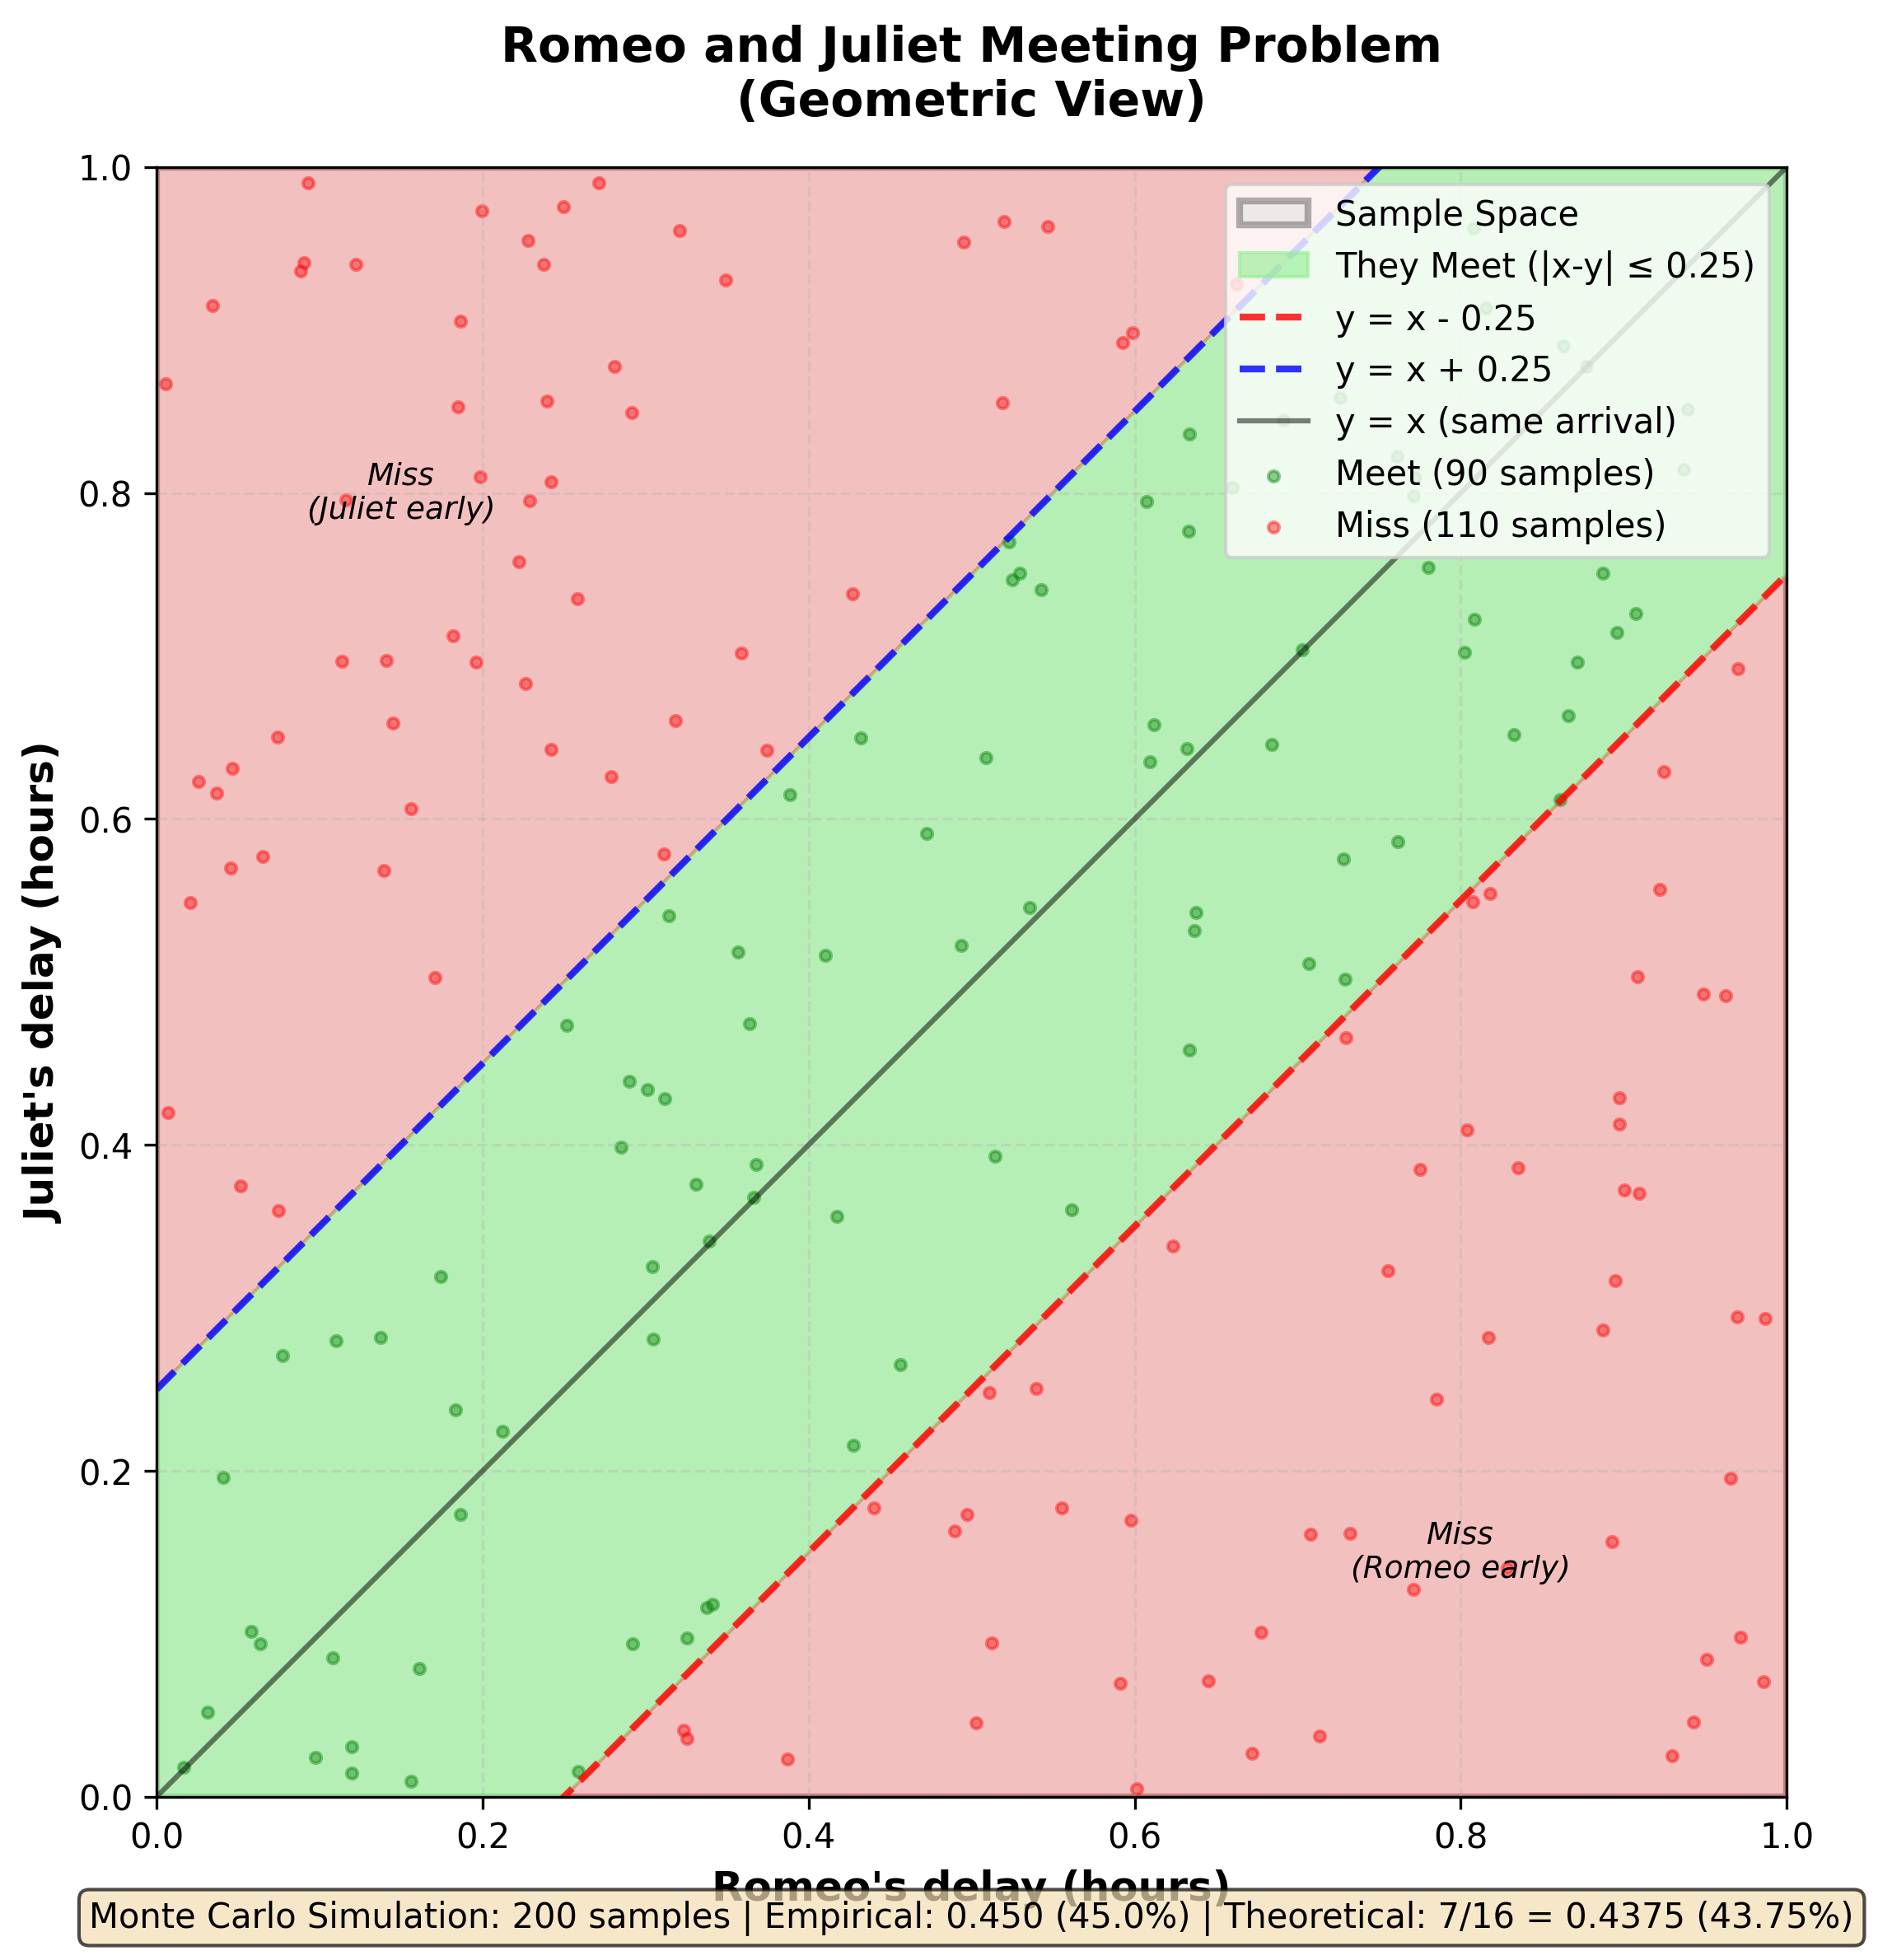
\includegraphics[width=0.8\textwidth]{romeo_juliet_probability.png}
    \caption{Romeo and Juliet meeting probability visualization showing the sample space (unit square), the meeting region (green band where $|x-y| \leq 0.25$), and miss regions (red triangles). The colored dots represent a Monte Carlo simulation with 200 random scenarios: green dots show cases where they meet, red dots show cases where they miss each other.}
    \label{fig:romeo_juliet}
\end{figure}

\begin{figure}[H]
    \centering
    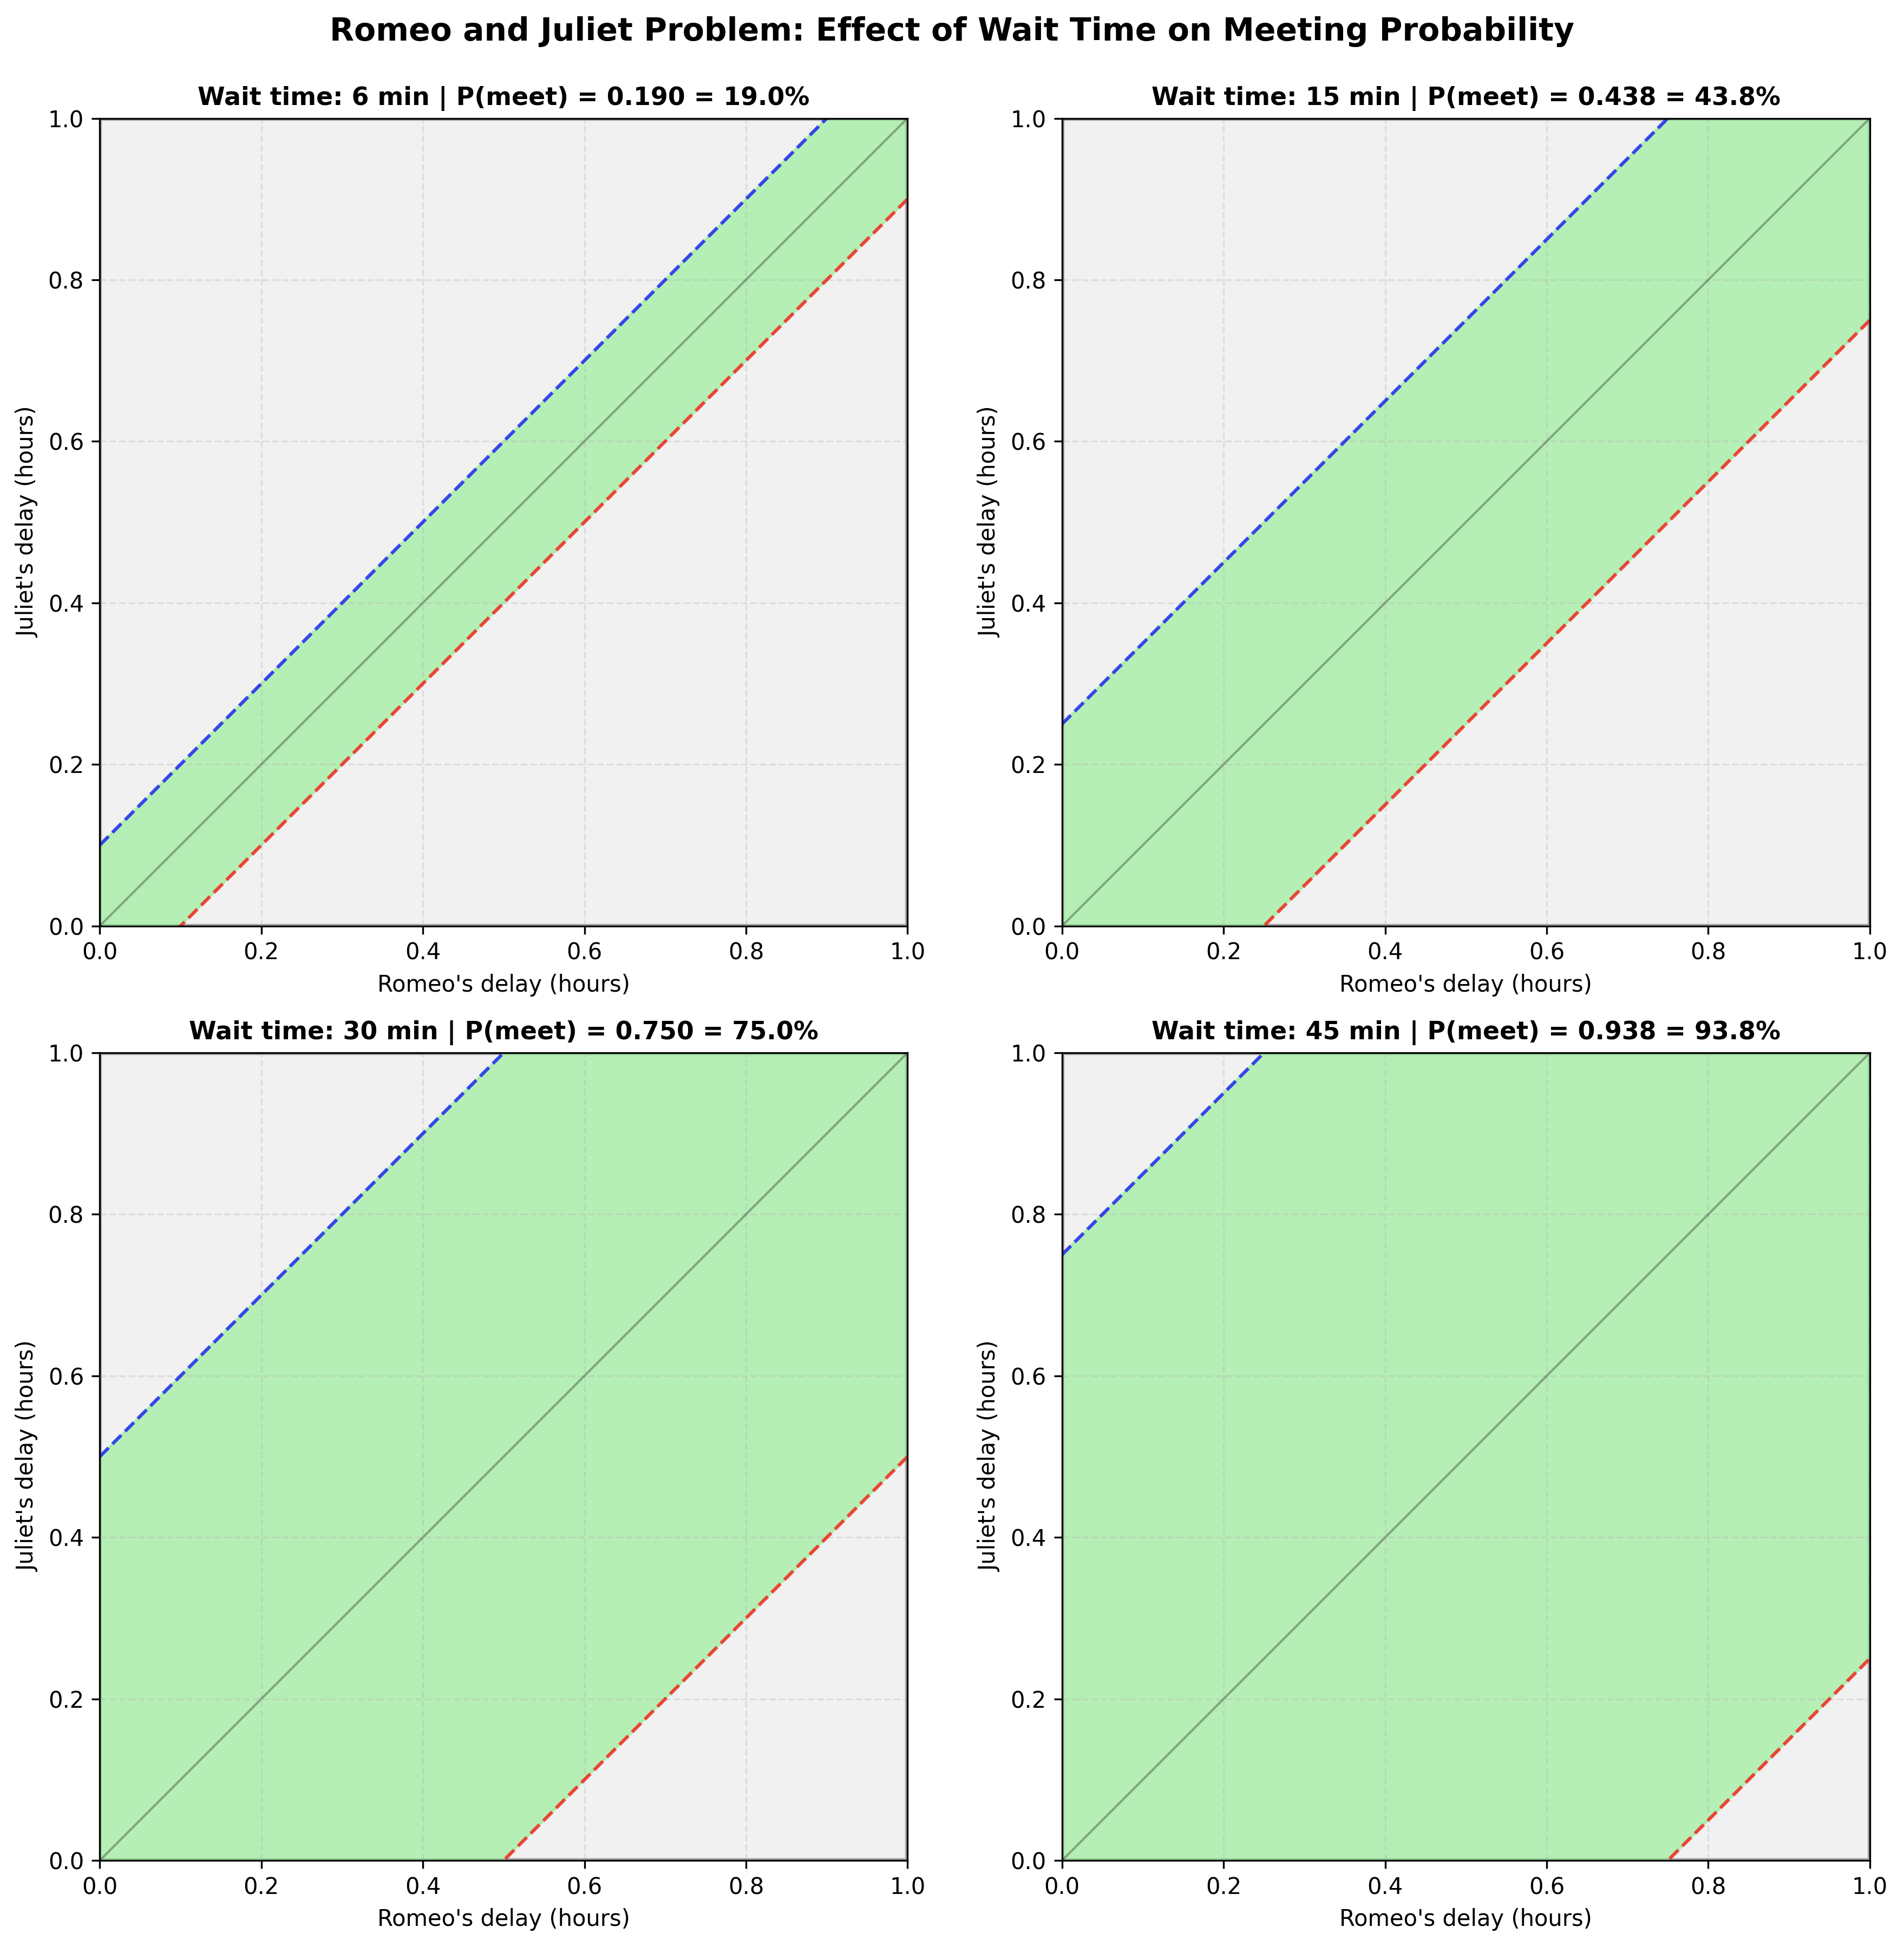
\includegraphics[width=\textwidth]{romeo_juliet_wait_times.png}
    \caption{Effect of different wait times on the probability of Romeo and Juliet meeting. The visualization shows how the meeting probability increases as the wait time increases from 6 minutes (10\%) to 45 minutes (75\%).}
    \label{fig:romeo_juliet_wait_times}
\end{figure}

\begin{keyconceptboxbreak}{Monte Carlo Simulation: Computing Probabilities Through Random Sampling}

\headingB{What is Monte Carlo Simulation?}

Monte Carlo simulation is a powerful computational technique that uses \textbf{random sampling} to solve problems and estimate probabilities—especially when exact mathematical solutions are difficult or impossible to find. The name comes from the famous Monte Carlo Casino in Monaco, reflecting the role of randomness in the method.

\headingB{The Core Idea}

Instead of calculating probability through mathematical formulas, we:
\begin{enumerate}
    \item \textbf{Simulate} the random experiment many times (thousands or millions)
    \item \textbf{Count} how often the event of interest occurs
    \item \textbf{Estimate} the probability as:
    \[
    P(\text{event}) \approx \frac{\text{Number of times event occurs}}{\text{Total number of simulations}}
    \]
\end{enumerate}

\headingB{Why Does This Work? The Law of Large Numbers}

The mathematical foundation is the \textbf{Law of Large Numbers}, which states:

\textit{As the number of independent trials of a random experiment increases, the observed relative frequency of an event approaches its true probability.}

In simple terms: If you flip a fair coin 10 times, you might get 7 heads. But if you flip it 10,000 times, you'll get very close to 5,000 heads (50\%). The more trials, the more accurate your estimate becomes.

\headingB{Monte Carlo for Romeo and Juliet Problem}

Let's see how Monte Carlo simulation works for our Romeo and Juliet meeting problem, where we calculated the theoretical probability as $\frac{7}{16} = 0.4375$ (43.75\%).

\textbf{Step-by-Step Process:}

\begin{enumerate}
    \item \textbf{Generate Random Arrival Times}
    \begin{itemize}
        \item For each simulation trial, randomly pick Romeo's delay: $x \sim \text{Uniform}(0, 1)$
        \item Randomly pick Juliet's delay: $y \sim \text{Uniform}(0, 1)$
        \item Each number is equally likely anywhere between 0 and 1 hour
    \end{itemize}

    \item \textbf{Check the Meeting Condition}
    \begin{itemize}
        \item Calculate the difference: $|x - y|$
        \item If $|x - y| \leq 0.25$ (within 15 minutes), they meet → count this as a success
        \item Otherwise, they miss each other
    \end{itemize}

    \item \textbf{Repeat Many Times}
    \begin{itemize}
        \item Run steps 1-2 for $N$ trials (e.g., $N = 10{,}000$)
        \item Keep track of successes (meetings) and failures (misses)
    \end{itemize}

    \item \textbf{Estimate the Probability}
    \[
    \hat{P}(\text{meet}) = \frac{\text{Number of meetings}}{N}
    \]
\end{enumerate}

\textbf{Example Results:}
\begin{itemize}
    \item With 100 simulations: might get 39 meetings → $\hat{P} = 0.39$ (39\%)
    \item With 1,000 simulations: might get 441 meetings → $\hat{P} = 0.441$ (44.1\%)
    \item With 10,000 simulations: might get 4,368 meetings → $\hat{P} = 0.4368$ (43.68\%)
    \item With 100,000 simulations: might get 43,742 meetings → $\hat{P} = 0.43742$ (43.742\%)
\end{itemize}

Notice how the estimate gets closer to the true value (0.4375) as we increase the number of simulations!

\headingB{Python Implementation}

Here's a complete Python program that implements Monte Carlo simulation for this problem:

\end{keyconceptboxbreak}

\begin{codeblock}{Python: Monte Carlo Simulation for Romeo and Juliet}
\begin{lstlisting}
import numpy as np
import matplotlib.pyplot as plt

def monte_carlo_romeo_juliet(n_simulations=10000, wait_time=0.25):
    """
    Monte Carlo simulation for Romeo and Juliet meeting problem.

    Parameters:
    -----------
    n_simulations : int
        Number of random trials to run
    wait_time : float
        How long they wait (in hours). Default: 0.25 (15 minutes)

    Returns:
    --------
    estimated_probability : float
        Estimated probability of meeting
    """
    # Step 1: Generate random arrival times
    # np.random.uniform(low, high, size) generates random numbers
    # uniformly distributed between 'low' and 'high'
    romeo_arrivals = np.random.uniform(0, 1, n_simulations)
    juliet_arrivals = np.random.uniform(0, 1, n_simulations)

    # Step 2: Check meeting condition for each pair
    # They meet if |romeo_time - juliet_time| <= wait_time
    time_differences = np.abs(romeo_arrivals - juliet_arrivals)
    they_meet = time_differences <= wait_time

    # Step 3: Count successes
    number_of_meetings = np.sum(they_meet)

    # Step 4: Calculate probability estimate
    estimated_prob = number_of_meetings / n_simulations

    return estimated_prob, romeo_arrivals, juliet_arrivals, they_meet

# Run the simulation
np.random.seed(42)  # For reproducible results
prob, romeo, juliet, meet = monte_carlo_romeo_juliet(10000)

# Display results
print(f"Monte Carlo Simulation Results:")
print(f"Number of simulations: 10,000")
print(f"Number of meetings: {np.sum(meet)}")
print(f"Estimated probability: {prob:.4f} ({prob*100:.2f}%)")
print(f"\nTheoretical probability: 7/16 = {7/16:.4f} ({7/16*100:.2f}%)")
print(f"Estimation error: {abs(prob - 7/16):.4f}")

# Visualize convergence: How estimate improves with more trials
def show_convergence():
    """Show how Monte Carlo estimate converges to true value."""
    sample_sizes = [10, 50, 100, 500, 1000, 5000, 10000, 50000]
    estimates = []

    for n in sample_sizes:
        prob, _, _, _ = monte_carlo_romeo_juliet(n)
        estimates.append(prob)

    # Plot
    plt.figure(figsize=(10, 6))
    plt.semilogx(sample_sizes, estimates, 'bo-', label='MC Estimate')
    plt.axhline(y=7/16, color='r', linestyle='--',
                label='True Probability (7/16)')
    plt.xlabel('Number of Simulations')
    plt.ylabel('Estimated Probability')
    plt.title('Monte Carlo Convergence')
    plt.grid(True, alpha=0.3)
    plt.legend()
    plt.show()

show_convergence()
\end{lstlisting}
\end{codeblock}

\begin{keyconceptboxbreak}{Understanding the Code}

\textbf{Key Python Concepts Used:}

\begin{enumerate}
    \item \texttt{np.random.uniform(0, 1, n)}: Generates $n$ random numbers uniformly distributed between 0 and 1. This simulates arrival times.

    \item \texttt{np.abs(array)}: Computes absolute value element-wise. We use this to find $|x - y|$ for all pairs.

    \item \texttt{array <= value}: Creates a boolean array (True/False values). Each element is True if the condition holds, False otherwise.

    \item \texttt{np.sum(boolean\_array)}: Counts how many True values exist. This gives us the number of meetings.
\end{enumerate}

\textbf{Why Monte Carlo is Powerful:}

\begin{itemize}
    \item \textbf{Versatility}: Works for problems where exact solutions are unknown or very complex
    \item \textbf{Intuitive}: Mirrors how we might test something in real life (run experiments)
    \item \textbf{Parallelizable}: Can run simulations simultaneously on multiple computers
    \item \textbf{Visualization}: Provides actual sample points we can plot and analyze
    \item \textbf{Validation}: Confirms theoretical results or finds errors in calculations
\end{itemize}

\textbf{Real-World Applications:}

\begin{itemize}
    \item \textbf{Finance}: Stock price modeling, option pricing, risk assessment
    \item \textbf{Physics}: Particle simulations, quantum mechanics computations
    \item \textbf{Engineering}: Reliability analysis, stress testing systems
    \item \textbf{Medicine}: Clinical trial design, drug dosage optimization
    \item \textbf{Machine Learning}: Training neural networks, reinforcement learning
    \item \textbf{Climate Science}: Weather prediction, climate change modeling
\end{itemize}

\textbf{Trade-offs:}

\begin{itemize}
    \item[$+$] Can solve very complex problems
    \item[$+$] Easy to implement and understand
    \item[$+$] Accuracy improves with more simulations
    \item[$-$] Requires many trials for high accuracy (computational cost)
    \item[$-$] Only gives approximate answers, not exact solutions
    \item[$-$] Need good random number generators
\end{itemize}

\end{keyconceptboxbreak}

\begin{definitionboxbreak}{Continuous Probability Models}
A continuous probability model involves a sample space $\Omega$ that contains uncountably many outcomes, typically corresponding to one or more continuous variables. In such models:
\begin{itemize}
    \item The probability of any single point is typically zero: $P(\{x\}) = 0$ for any $x \in \Omega$
    \item Probabilities are assigned to intervals or regions rather than individual points
    \item The probability law is often specified through a probability density function (PDF)
\end{itemize}
\end{definitionboxbreak}

\subsubsection{Properties of Probability Laws}

From the axioms of probability, we can derive several important properties that hold for any probability law:
\begin{itemize}
    \item \textbf{Complement Rule:} For any event \(A\), the probability of its complement \(A^c\) is given by:
    \[ P(A^c) = 1 - P(A) \]
    \item \textbf{Monotonicity:} If \(A \subseteq B\), then:
    \[ P(A) \leq P(B) \]
    \item \textbf{Inclusion-Exclusion Principle:} For any two events \(A\) and \(B\):
    \[ P(A \cup B) = P(A) + P(B) - P(A \cap B) \]
    \item \textbf{Union Bound:} For any events \(A_1, A_2, \ldots, A_n\):
    \[ P\left(\bigcup_{i=1}^{n} A_i\right) \leq \sum_{i=1}^{n} P(A_i) \]
\end{itemize}

\subsection{The Two-Stage Framework of Probability}

Applying probability theory to real-world uncertainty involves two distinct stages:

\headingB{Stage 1: Model Construction (Art)}
\begin{itemize}
    \item Build a probabilistic model by specifying a sample space and probability law
    \item No rigid rules—must satisfy only the three axioms
    \item Reasonable people may disagree on the "best" model
    \item Often involves tradeoffs: accuracy vs. simplicity vs. tractability
    \item May intentionally use "incorrect" but useful models
\end{itemize}

\headingB{Stage 2: Mathematical Analysis (Science)}
\begin{itemize}
    \item Work within the fully specified model
    \item Calculate probabilities of events or derive properties
    \item Governed strictly by logic and probability axioms
    \item All questions have precise answers—only skill required
    \item May be complex, but never ambiguous
\end{itemize}

\begin{exampleboxbreak}{Two-Stage Framework in Action}

\headingB{Scenario:} A tech company wants to model user clicks on their website.

\headingB{Stage 1 — Model Construction:}

Three data scientists propose different models:

\textbf{Model A (Simple):}
\begin{itemize}
    \item Sample space: $\Omega = \{\text{Click}, \text{No Click}\}$
    \item Probability law: $P(\text{Click}) = 0.15$ (based on historical average)
    \item \textit{Justification:} Simple, easy calculations, captures overall behavior
\end{itemize}

\textbf{Model B (Time-Aware):}
\begin{itemize}
    \item Sample space: $\Omega = \{\text{Click}, \text{No Click}\} \times \{\text{Morning}, \text{Afternoon}, \text{Evening}\}$
    \item Different click probabilities for different times of day
    \item \textit{Justification:} More accurate, accounts for daily patterns
\end{itemize}

\textbf{Model C (Complex):}
\begin{itemize}
    \item Sample space includes user demographics, previous behavior, device type, etc.
    \item Probability law based on machine learning model
    \item \textit{Justification:} Most accurate, but computationally expensive
\end{itemize}

\textit{Who is right?} All three! The choice depends on:
\begin{itemize}
    \item What questions need answering
    \item Available computational resources
    \item Required accuracy level
    \item Time constraints
\end{itemize}

\headingB{Stage 2 — Mathematical Analysis:}

Once Model A is chosen, questions have definite answers:
\begin{itemize}
    \item Q: ``What's the probability of 3 clicks out of 10 users?''
    \item A: Using binomial formula: $P(X=3) = \binom{10}{3}(0.15)^3(0.85)^7 = 0.1298$
\end{itemize}

No ambiguity here—the model determines the answer uniquely.

\end{exampleboxbreak}

\begin{exampleboxbreak}{The Danger of Ambiguous Models}

\headingB{The Birthday Paradox "Paradox"}

\textbf{Claim:} ``In a room of 30 people, what's the probability two share a birthday?''

\textbf{Two analysts disagree:}

\textit{Analyst 1:} ``The probability is about 70\%—I calculated it using the standard birthday problem formula.''

\textit{Analyst 2:} ``No, it's much lower! I got 7.7\%.''

\headingB{What went wrong?}

\textbf{Hidden Model Assumptions:}

\textit{Analyst 1's Model:}
\begin{itemize}
    \item Event: ``At least two people share some birthday''
    \item Assumes: All birthdays equally likely, no twins, 365 days/year
    \item Answer: $P \approx 0.706$ (70.6\%)
\end{itemize}

\textit{Analyst 2's Model:}
\begin{itemize}
    \item Event: ``At least one person shares \textit{my specific} birthday''
    \item This is a different question!
    \item Answer: $P = 1 - (364/365)^{29} \approx 0.077$ (7.7\%)
\end{itemize}

\headingB{The Lesson:}

There's no "paradox"—just \textbf{poorly specified models}. Once we clarify:
\begin{itemize}
    \item What exactly is the sample space?
    \item What precisely is the event of interest?
    \item What are our assumptions?
\end{itemize}

The apparent contradiction disappears. Stage 1 (model specification) must be unambiguous before Stage 2 (calculation) can proceed.

\end{exampleboxbreak}

\begin{keyconceptboxbreak}{Avoiding Probability "Paradoxes"}

\textbf{Key Insight:} Probability theory contains many apparent "paradoxes" where different methods seem to give different answers to the same question.

\textbf{The Truth:} These paradoxes invariably reflect:
\begin{itemize}
    \item Poorly specified probabilistic models
    \item Ambiguous problem statements
    \item Hidden or unstated assumptions
    \item Different interpretations of the same verbal description
\end{itemize}

\textbf{Resolution Strategy:}
\begin{enumerate}
    \item \textbf{Explicitly state} the sample space $\Omega$
    \item \textbf{Precisely define} all events of interest
    \item \textbf{Clearly specify} the probability law and its assumptions
    \item \textbf{Verify} that all parties agree on the model before calculating
\end{enumerate}

Once Stage 1 is unambiguous, Stage 2 has no room for disagreement—mathematics is deterministic.

\end{keyconceptboxbreak}

\begin{funfactsbreak}{Markov Chains: When the Past Doesn't Matter}

\headingB{The Memoryless Property}

Imagine a drunk person wandering on a street, taking random steps left or right. Where they go next depends only on where they are \textit{right now}—not on how they got there. This is the essence of a \textbf{Markov chain}!

\headingB{What is a Markov Chain?}

A Markov chain is a mathematical system that transitions from one state to another according to certain probabilistic rules. The key property:
\begin{center}
\textit{``The future depends only on the present, not on the past.''}
\end{center}

Formally: $P(\text{Next state} \mid \text{Current state, Past states}) = P(\text{Next state} \mid \text{Current state})$

\headingB{Real-World Examples:}

\begin{itemize}
    \item \textbf{Weather Prediction:} If it's sunny today, there's a 70\% chance it's sunny tomorrow and 30\% chance of rain—regardless of whether it rained last week.

    \item \textbf{Google's PageRank:} The algorithm that ranks web pages models a random web surfer clicking links. The probability of visiting a page depends only on the current page, not the browsing history.

    \item \textbf{Stock Prices (Efficient Market Hypothesis):} Some models assume tomorrow's price depends only on today's price, not on the entire price history.

    \item \textbf{Board Games:} In Monopoly, your next position depends only on where you are now and the dice roll—not on your previous moves.

    \item \textbf{Text Generation (AI):} Simple text prediction models (like early autocomplete) choose the next word based only on the current word.
\end{itemize}

\headingB{A Simple Example: The Weather Model}

Suppose we have two states: Sunny (S) and Rainy (R). The transition probabilities are:
\begin{itemize}
    \item If today is Sunny: 80\% chance tomorrow is Sunny, 20\% chance of Rain
    \item If today is Rainy: 50\% chance tomorrow is Sunny, 50\% chance of Rain
\end{itemize}

We can represent this as a \textbf{transition matrix}:
\[
P = \begin{pmatrix}
0.8 & 0.2 \\
0.5 & 0.5
\end{pmatrix}
\]
where rows represent current state and columns represent next state.

\begin{figure}[H]
    \centering
    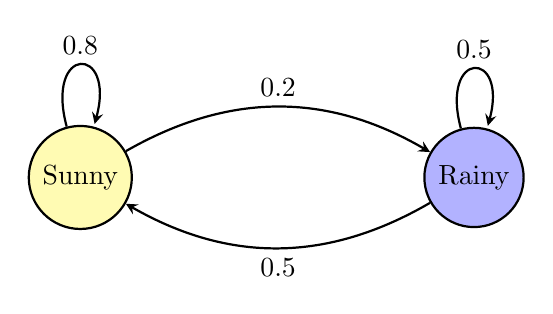
\begin{tikzpicture}[->, >=stealth, auto, node distance=3cm, thick]
        % States
        \node[circle, draw, fill=yellow!30, minimum size=1.2cm] (S) {Sunny};
        \node[circle, draw, fill=blue!30, minimum size=1.2cm, right of=S, node distance=5cm] (R) {Rainy};

        % Transitions
        \path (S) edge [loop above] node {0.8} (S)
              (S) edge [bend left] node {0.2} (R)
              (R) edge [bend left] node {0.5} (S)
              (R) edge [loop above] node {0.5} (R);
    \end{tikzpicture}
    \caption{Markov chain state diagram for the weather model}
    \label{fig:markov_weather}
\end{figure}

\headingB{Interesting Fact:}

Many Markov chains reach a \textbf{steady state} (equilibrium) where the long-term probabilities stabilize. For our weather example, no matter what the weather is today, after many days the probability converges to approximately 71.4\% Sunny and 28.6\% Rainy!

\headingB{Modern Applications:}

\begin{itemize}
    \item \textbf{Machine Learning:} Hidden Markov Models (HMMs) for speech recognition
    \item \textbf{Finance:} Modeling credit rating transitions
    \item \textbf{Biology:} DNA sequence analysis
    \item \textbf{Queueing Theory:} Modeling customer service systems
    \item \textbf{Physics:} Statistical mechanics and thermodynamics
\end{itemize}

Named after Russian mathematician Andrey Markov (1856-1922), who first studied these chains in the early 1900s while analyzing the patterns of vowels and consonants in Russian literature!

\end{funfactsbreak}

\section{Exercises}

